\documentclass[a4paper,10pt]{article}
\usepackage[spanish]{babel}
\usepackage[utf8]{inputenc}
\usepackage{bm} %letras griegas en negrita (uso: \bm{\alpha})
\usepackage{wrapfig}
\usepackage{graphicx}
\usepackage{float}
\usepackage{amsmath}
\usepackage{listings}
\spanishdecimal{.}
\setlength{\headheight}{30pt}
\usepackage{amsmath,amsfonts,latexsym,cancel,textcomp,anysize,color,subfigure}
\marginsize{1.5cm}{1cm}{0.3cm}{0.3cm} %izq,der,sup,inf
\parindent=0mm %sangría
\parskip=3mm %espacio entre párrafos
\usepackage{fancyhdr}
\pagestyle{fancy}
\def\changemargin#1#2{\list{}{\rightmargin#2\leftmargin#1}\item[]}
\let\endchangemargin=\endlist
\title{Manual de Apache Spark}
\author{Adrián García Novoa}
\date{Diciembre 2020}
\usepackage{hyperref}
\hypersetup{
    colorlinks=true,
    linkcolor=black,
    filecolor=magenta,      
    urlcolor=cyan,
}
\urlstyle{same}

\begin{document}
\begin{figure}[H]
\begin{center}

\includegraphics[width=340pt]{./fotos/introduccion/Apache_Spark_logo.jpg}
\end{center}
\end{figure}
\clearpage

\lhead{\leftmark}
\chead{}
\rhead{Manual Apache Spark}
\renewcommand{\headrulewidth}{0.4pt}
\lfoot{}
\cfoot{\thepage}
\rfoot{}
\renewcommand{\footrulewidth}{0.4pt}

\tableofcontents
\clearpage

\lhead{\leftmark}
\rhead{Manual Apache Spark}

\section{Introducción}

La finalidad de este documento sera la instalación y configuración de todas las herramientas necesarias para la programación en Apache Spark tanto en Python, como en Scala. 

Como extra, tendremos una sección donde podremos ver como trabajar con Apache Spark por medio del procesamiento en la nube.
	
\clearpage		

\section{Instalación y Configuración en Windows 10}

\subsection{Requisitos}

Sistema con Windows 10 de 64bits

Descompresor de archivos, nosotros utilizaremos 7-Zip

 \clearpage

\subsection{Java JDK}

El Java JDK es el Java Development Kit, que traducido al español significa, Herramientas de desarrollo para Java. Aquí nos encontraremos con el compilador javac que es el encargado de convertir nuestro código fuente (.java) en bytecode (.class), el cual posteriormente sera interpretado y ejecutado en la JVM, Java Virtual Machine por sus siglas en ingles, que nuevamente en español significa, La Maquina Virtual de Java. 

Puede que nos suene mas Java JRE, este es el Java Runtime Environment, que en español significa, Entorno de Ejecución de Java. En palabras del propio portal de Java es la implementación de la Máquina virtual de Java que realmente ejecuta los programas de Java, esto quiere decir que aquí encontraremos todo lo necesario para ejecutar nuestras aplicaciones escritas en Java. 

Normalmente el JRE esta destinado a usuarios finales que no requieren el JDK, pues a diferencia de este, no contiene los programas necesarios para crear aplicaciones en el lenguaje Java, es así, que el JRE se puede instalar sin necesidad de instalar el JDK, pero al instalar el JDK, este siempre cuenta en su interior con el JRE.

\subsubsection{Descarga}

Si vamos a la web oficial de Oracle para la descarga de Java (\href{https://www.oracle.com/es/java/technologies/javase/javase-jdk8-downloads.html}{pagina oficial}) e intentamos descargarlo, nos obligara a crearnos una cuenta. Para evitar esto descargaremos la version libre de Java, OpenJDK. Accederemos a través de la siguiente dirección:

\begin{center}
\href{https://openjdk.java.net/}{https://openjdk.java.net/} 
\end{center}


Como podemos ver en las siguientes imágenes, en el segundo párrafo de la pagina principal, donde empieza con Download, haremos click  en \textit{jdk.java.net/15}. Esto nos llevara a la pagina de descargas, donde veremos versiones para los distintos sistemas operativos. En nuestro caso seleccionaremos la version de Windows/x64.

\begin{figure}[h]
\centering
\subfigure[Pagina principal]{
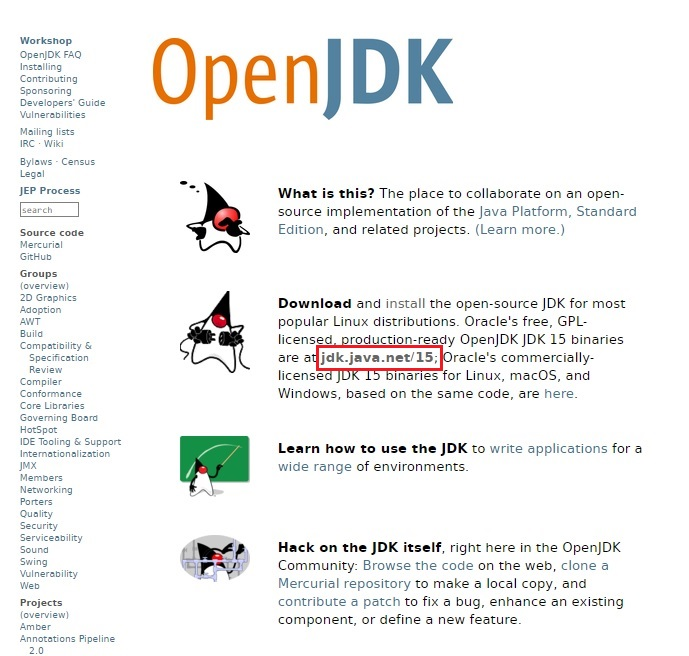
\includegraphics[width=0.45\textwidth]{./fotos/introduccion/24 - openjdk (V).jpg}}
\subfigure[Pagina de descargas]{
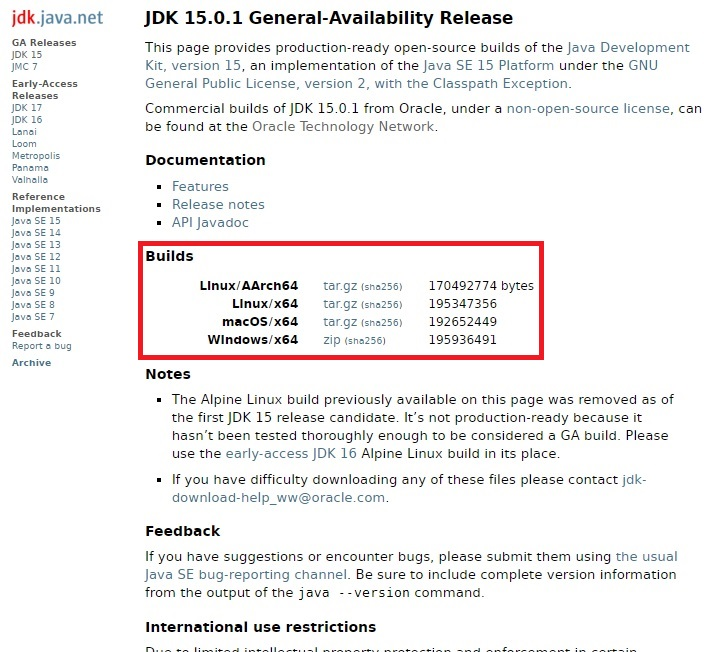
\includegraphics[width=0.45\textwidth]{./fotos/introduccion/25 - openjdk (V).jpg}}
\end{figure}
 
\clearpage

\subsubsection{Instalacion}

Una vez tengamos descargado nuestro OpenJDK, en nuestra carpeta de Descargas veremos que se trata de un archivo zip. Lo que primero que debemos hacer para instalarlo sera crear una carpeta en la raiz de nuestro disco duro (C:/) que se llame 'java'. Lo siquiente sera descomprimir el archivo descargado dentro de esa carpeta de manera que la ruta al contenido de Java JDK quedara en \textit{C:/java/jdk-15.0.1}

En la siguiente imagen podemos ver como debería quedarnos:

\begin{figure}[H]
\begin{center}
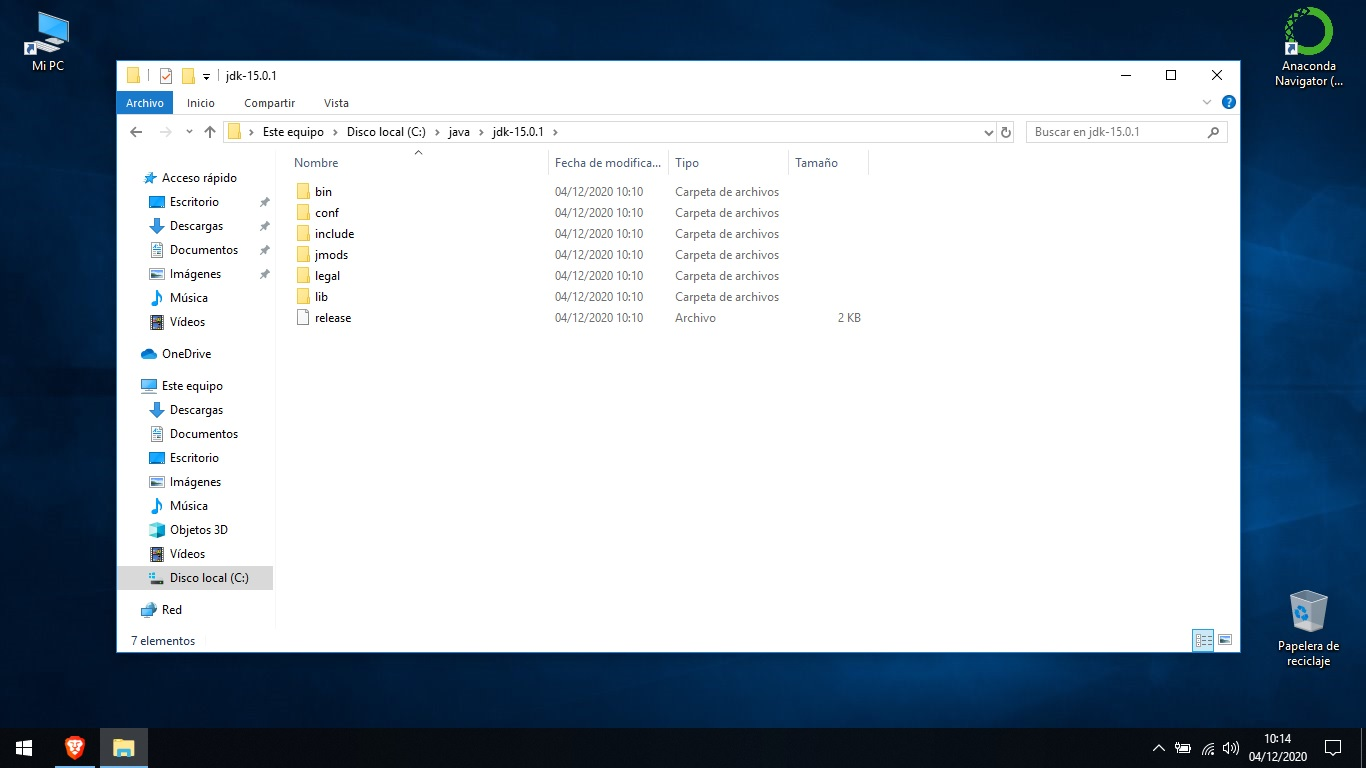
\includegraphics[width=450pt]{./fotos/introduccion/6 - Java.jpg}
\end{center}
\end{figure}

\clearpage

\subsubsection{Variables de entorno}

Seguramente muchos nunca hayan escuchado este termino. Para que se entienda de una manera sencilla, una variable de entorno no es mas que, una palabra, o un texto facilmente recordable que nos permitirá acceder a rutas mas complejas de forma mas sencilla. En el caso de Java por ejemeplo, sera mucho mas sencillo recordar 'java' que la ruta a la carpeta donde lo hemos instalado (\textit{C:/java/jdk-15.0.1}). Ademas, las variables de entorno facilitan al resto de programas con dependencias externas conocer la dirección donde se encuentran estas.

En este caso, deberemos crear la variable de entorno JAVA\_HOME y actualizar la variable de entorno PATH. La primera se utilizará para que Java sepa dónde se encuentra la instalación de Java JDK y la segunda es para poder ejecutar los comandos de Java (como javac, java, etc) desde cualquier lugar, como desde la consola del sistema. 

\textbf{JAVA\_HOME}

Hacemos click en inicio y escribiremos 'Editar las variables de entorno del sistema' como en la siguiente imagen:

\begin{figure}[H]
\begin{center}
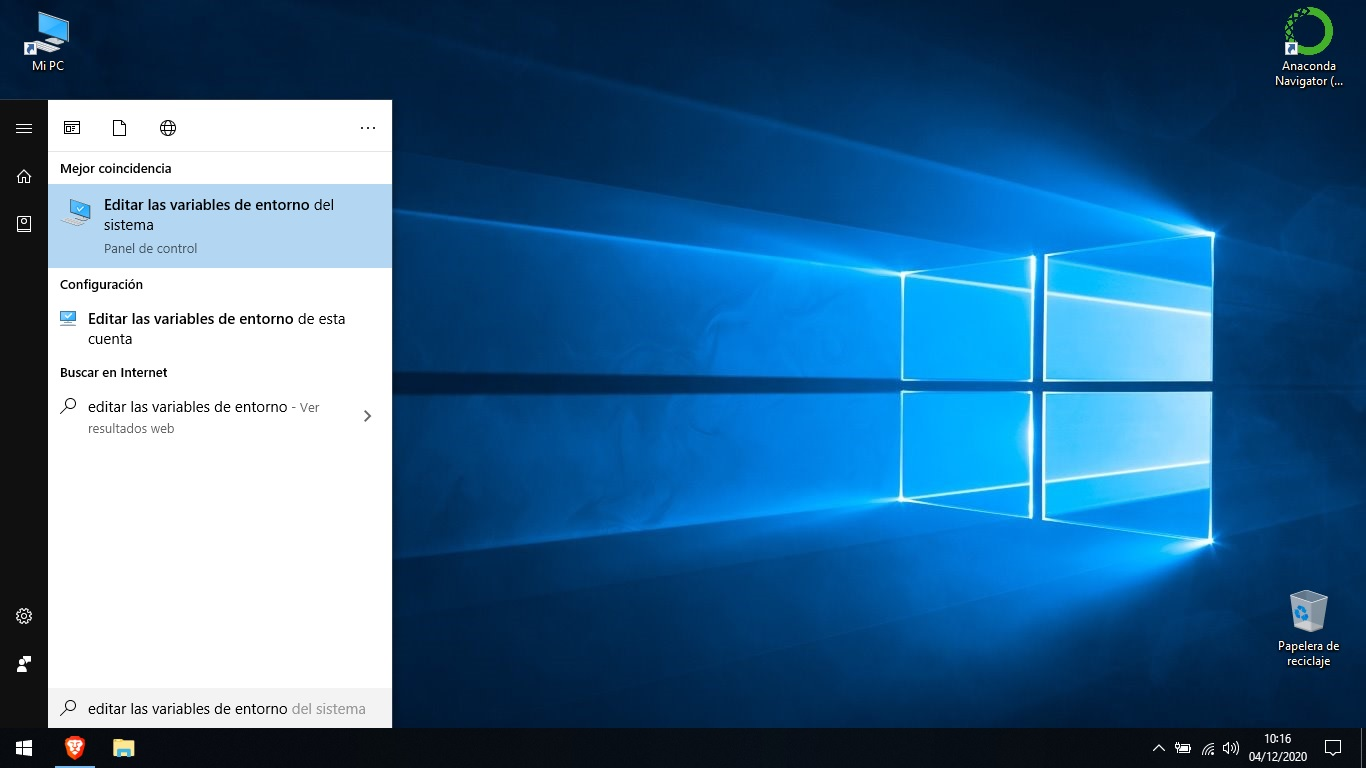
\includegraphics[width=425pt]{./fotos/introduccion/7 - Java.jpg}
\end{center}
\end{figure}

Al abrir el editor veremos que se abre la ventana de Propiedades del sistema. Hacemos click en la pestaña de 'Opciones avanzadas' y abajo hacemos click en 'Variables de entorno' como en la siguiente imagen:

\begin{figure}[H]
\begin{center}
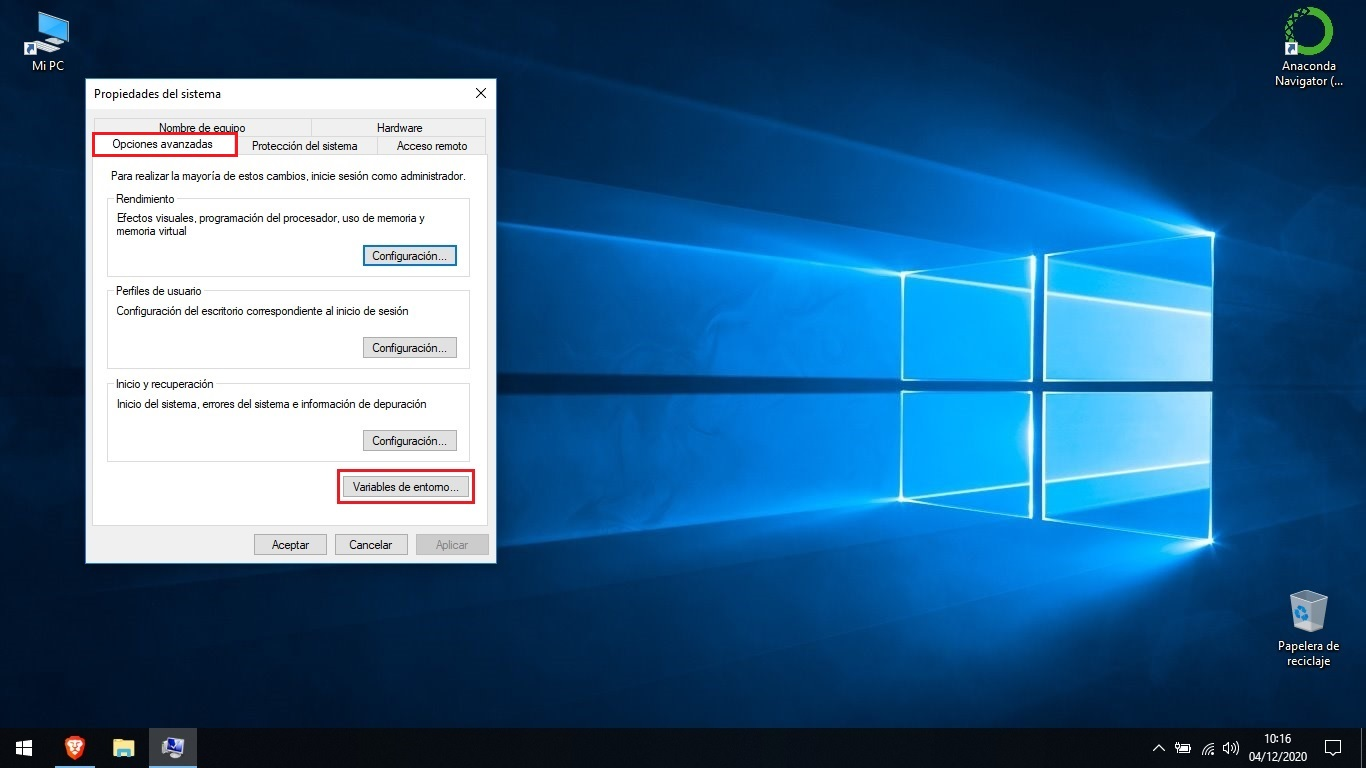
\includegraphics[width=425pt]{./fotos/introduccion/8 - Java (V).jpg}
\end{center}
\end{figure}

En la ventana que se nos ha abierto veremos dos recuadros. En uno pondrá \textit{Variables de usuario} y en el de debajo \textit{Variables del sistema}. Lo mas recomendable es crear las variables de entorno para el sistema, con el fin de que cualquier usuario tenga acceso a la ejecución de java. 

Entonces en el grupo de Variables del sistema hacemos click en el botón 'Nueva'.

\begin{figure}[H]
\begin{center}
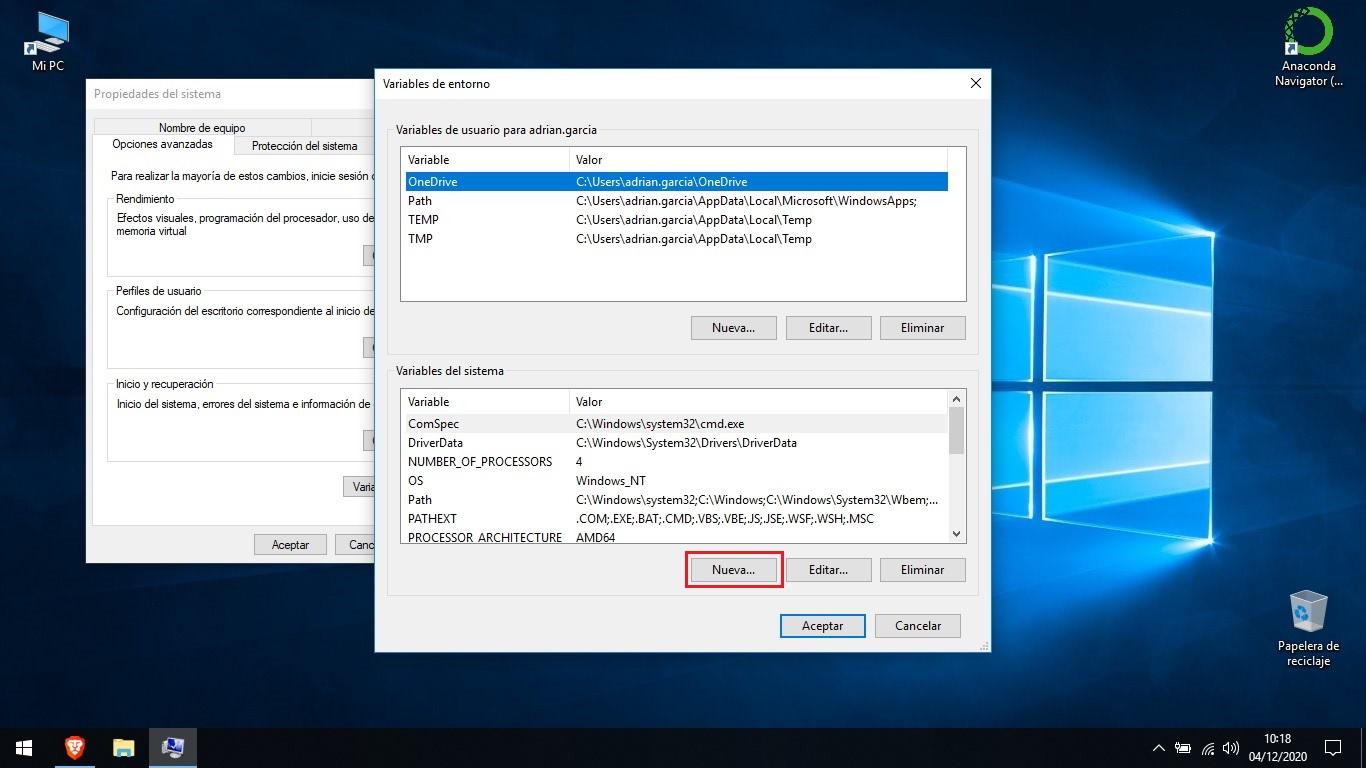
\includegraphics[width=450pt]{./fotos/introduccion/9 - Java (V).jpg}
\end{center}
\end{figure}

En el nombre escribiremos 'JAVA\_HOME', mientras que en valor la variable escribiremos la ruta donde se instalo el Java JDK, en nuestro caso será \textit{C:/java/jdk-11.0.2}

\begin{figure}[H]
\begin{center}
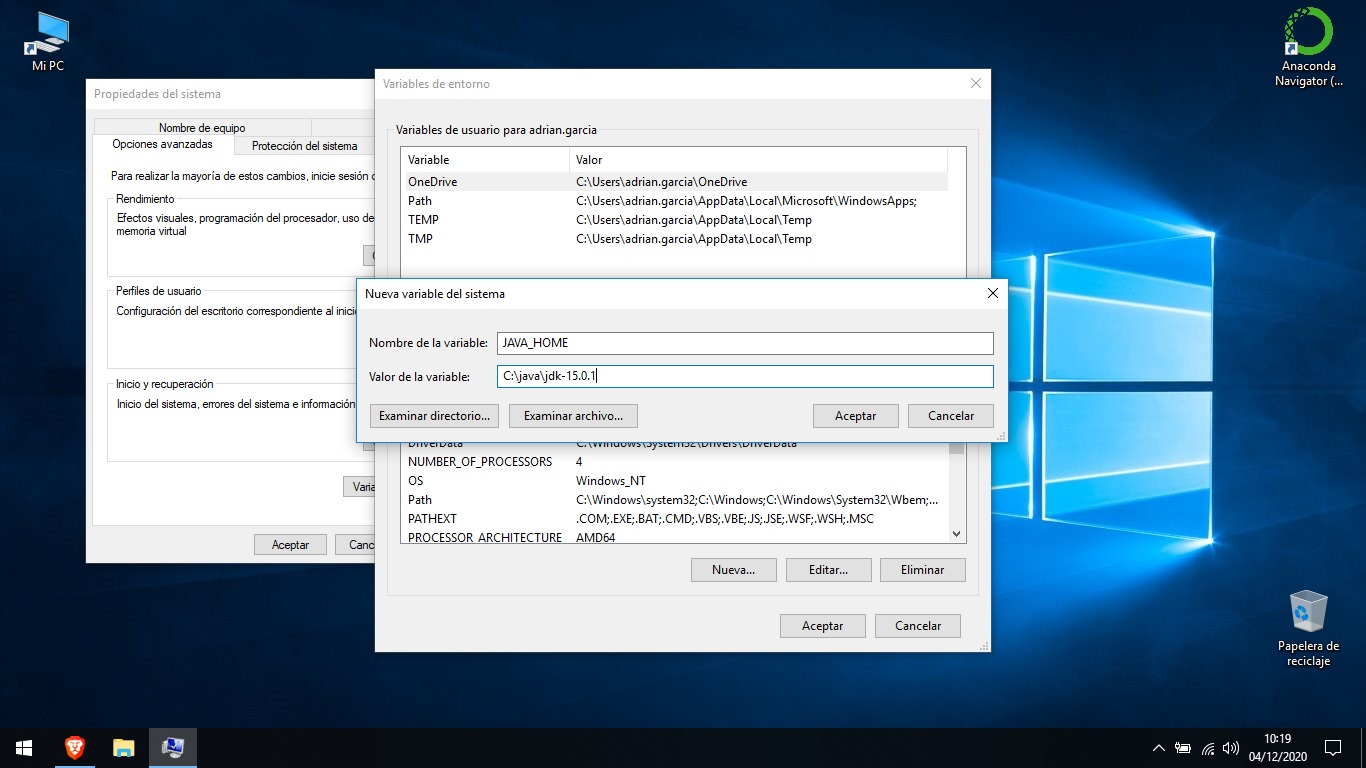
\includegraphics[width=450pt]{./fotos/introduccion/10 - Java.jpg}
\end{center}
\end{figure}

Hacemos clic en aceptar.

\clearpage

Debería quedarnos de la siguiente manera:

\begin{figure}[H]
\begin{center}
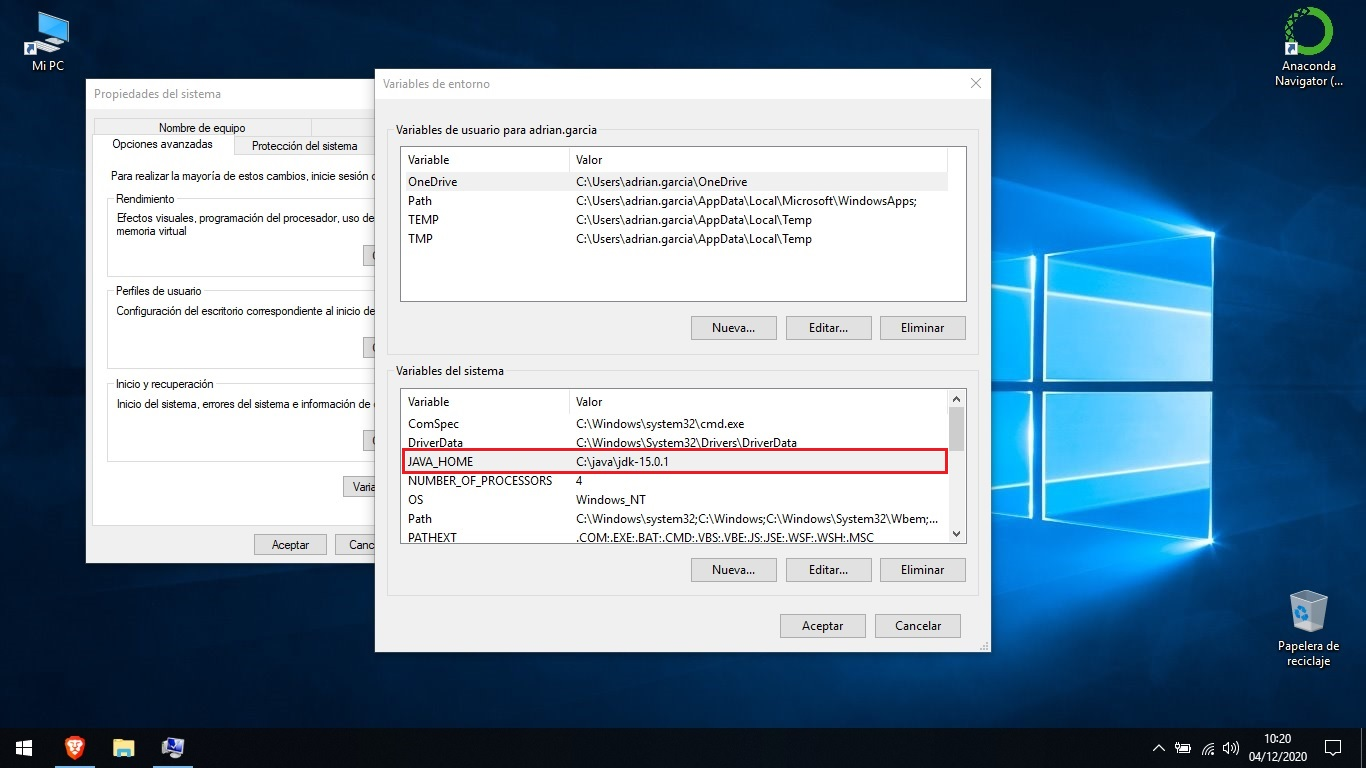
\includegraphics[width=500pt]{./fotos/introduccion/11 - Java (V).jpg}
\end{center}
\end{figure}

$\bullet$ PATH 

Si por alguna razón no tienes abierta la ventana de variables de entorno, repite los pasos anteriores. En este caso vamos a editar la variable Path que ya existe dentro de variables del sistema. La seleccionamos y le damos a editar:

\begin{figure}[H]
\begin{center}
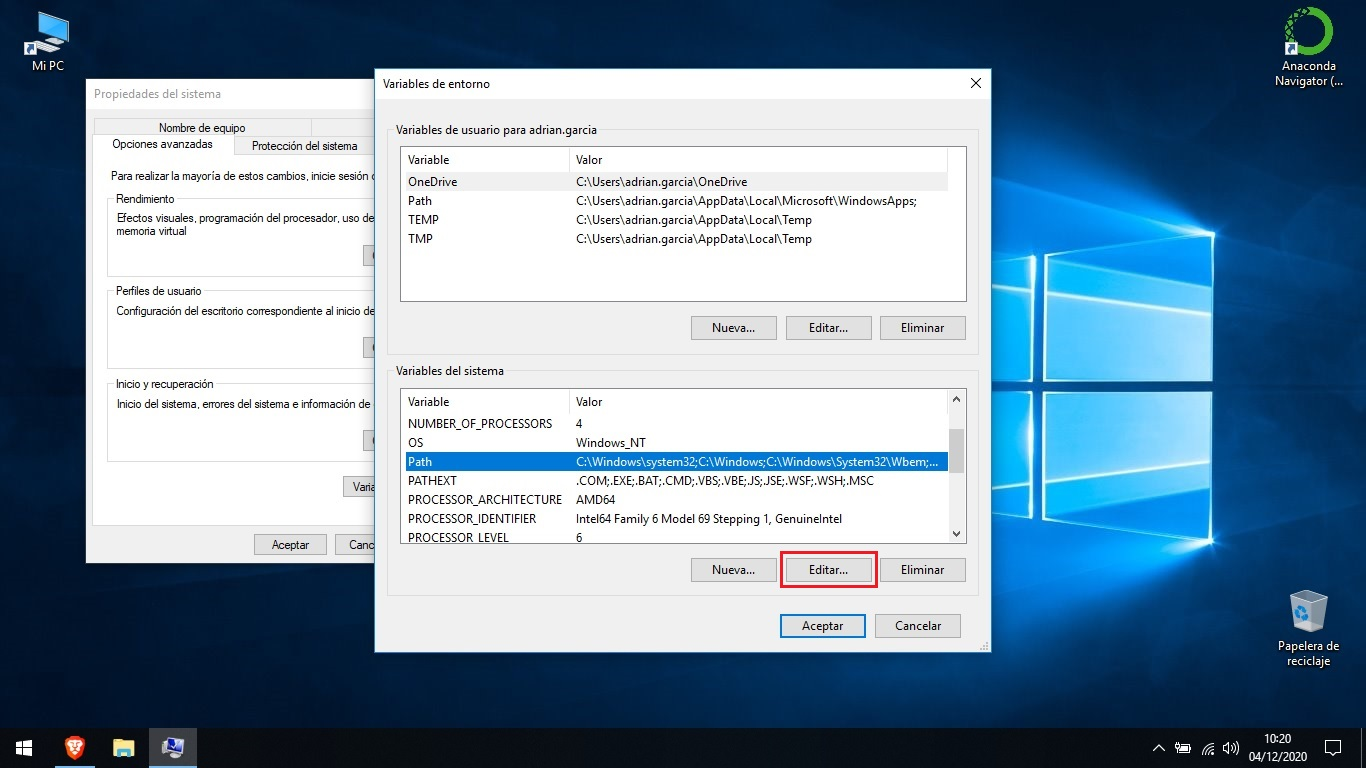
\includegraphics[width=500pt]{./fotos/introduccion/12 - Java (V).jpg}
\end{center}
\end{figure}

\clearpage

Podrás ver todos los valores que tiene por defecto la variable Path. No los modifiques o elimines, solo haz click en 'Nuevo' 

\begin{figure}[H]
\begin{center}
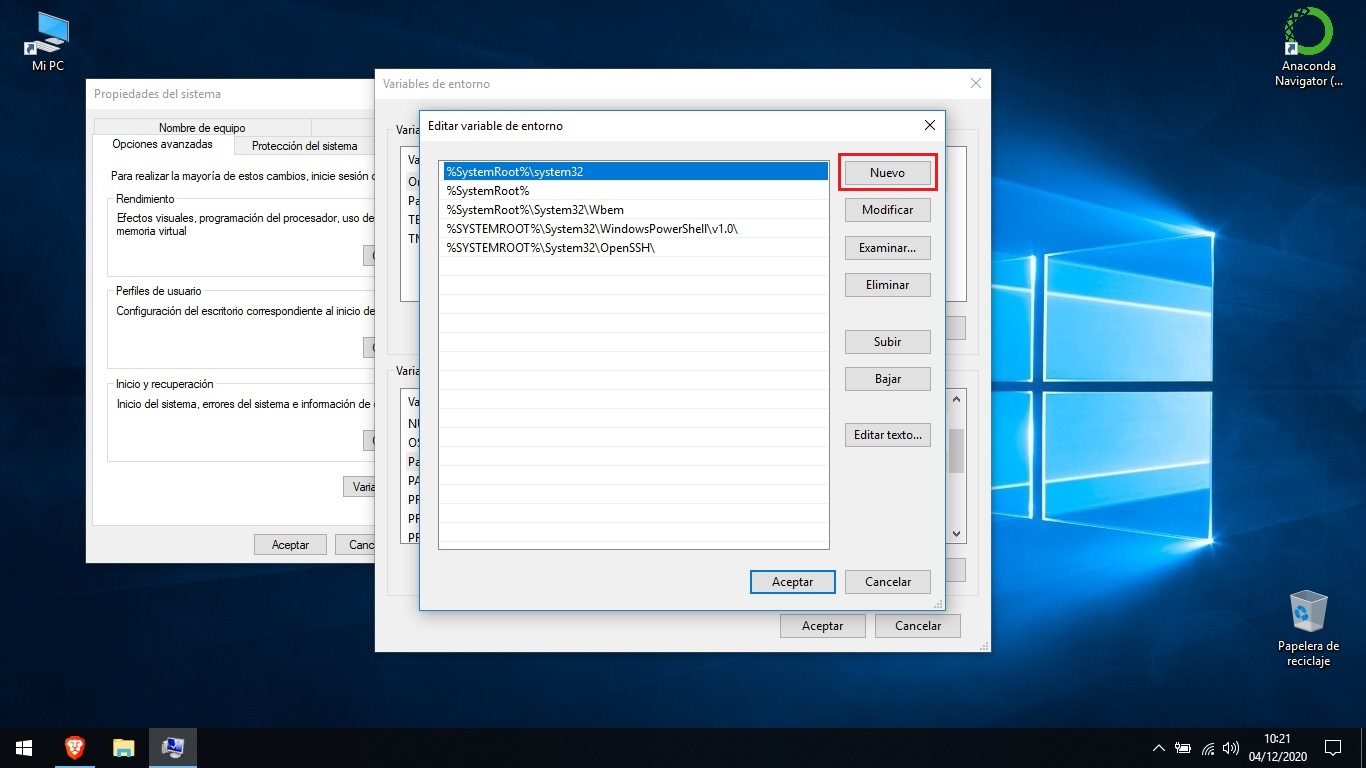
\includegraphics[width=500pt]{./fotos/introduccion/13 - Java (V).jpg}
\end{center}
\end{figure}

Escribiremos la ruta a la instalación de java, pero en este caso direccionandolo a la carpeta bin. Si has seguido todos los pasos hasta aquí, la ruta sera \textit{C:/java/jdk-11.0.2/bin}

\begin{figure}[H]
\begin{center}
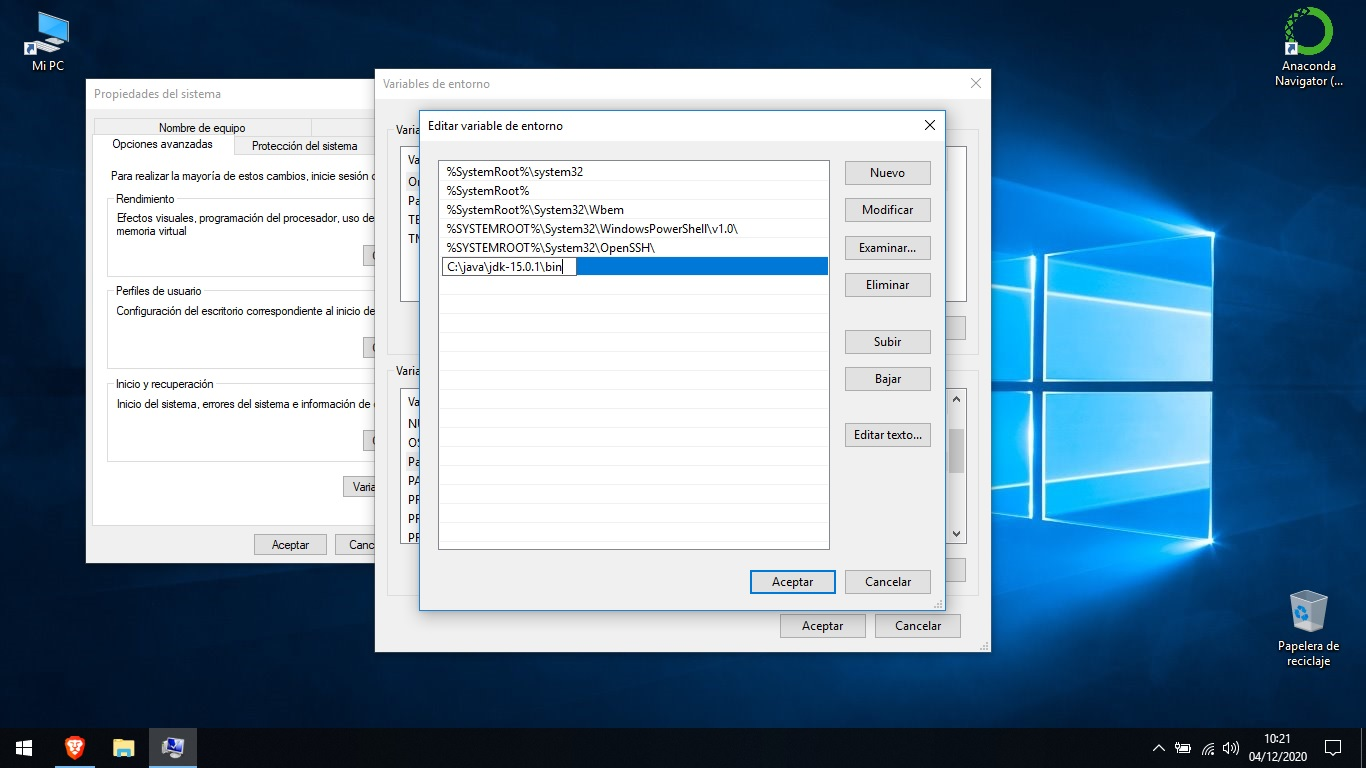
\includegraphics[width=500pt]{./fotos/introduccion/14 - Java.jpg}
\end{center}
\end{figure}

Aceptamos en la ventana de Path y volvemos a aceptar en la ventana de variables de entorno y en propiedades del sistema.

\clearpage

Ahora solo nos quedara comprobar que java esta correctamente instalado y las variables de entorno han sido correctamente configuradas. Para ello, como cuando abrimos el editor de variables de entorno, hacemos click en inicio y ahora escribiremos \textit{cmd} abriendo el programa \textbf{Símbolo del sistema}. En la ventana de comandos escribiremos \textbf{java -version} y deberíamos obtener el siguiente resultado:

\begin{figure}[H]
\begin{center}
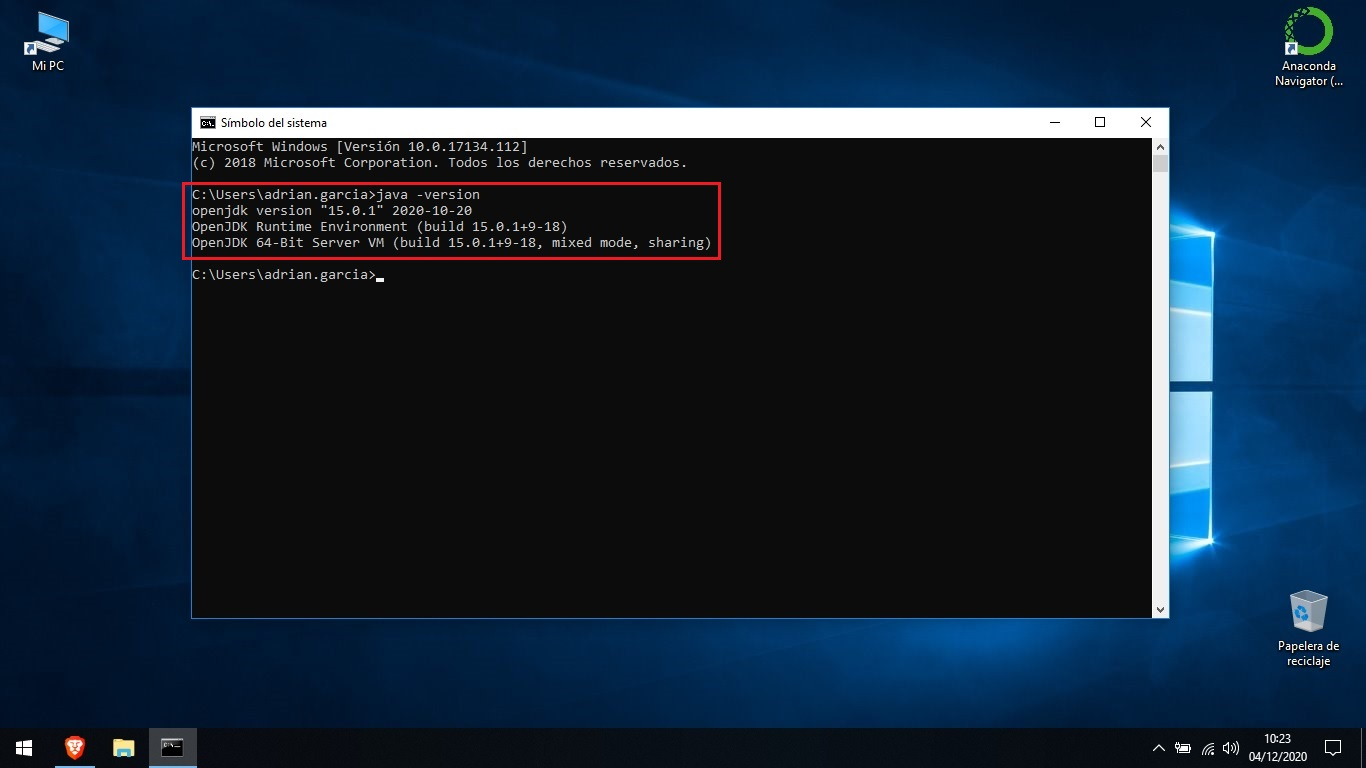
\includegraphics[width=500pt]{./fotos/introduccion/15 - Java (V).jpg}
\end{center}
\end{figure}

Como hemos podido comprobar, al introducir el termino \textit{java}, gracias a las variables de entorno, windows sabe la ruta a la que se tiene que dirigir. Y con el argumento \textit{--version} ejecuta la comprobación de la version instalada.

Con esto ya podemos decir que tenemos Java instalado y configurado en nuestro sistema. 

\clearpage

\subsection{Anaconda}

Anaconda es una solución flexible de código abierto que proporciona las utilidades para crear, distribuir, instalar, actualizar y administrar software de manera multiplataforma. Ademas nos facilita la gestión de múltiples entornos de datos que se pueden mantener y ejecutar por separado sin interferencias entre sí.
 
Nos va a servir para el procesamiento de datos a gran escala, el análisis predictivo y la informática científica, que tiene como objetivo simplificar la gestión de empaquetado y distribución. Esta es quizás la Suite más completa para la Ciencia de datos con Python y que nos brinda una gran cantidad de funcionalidades que nos van a permitir desarrollar aplicaciones de una manera más eficiente, rápida y sencilla. 


\subsubsection{Descarga}

El primero paso sera ir a la web oficial de Anaconda:
\begin{center}
\href{https://www.anaconda.com/}{https://www.anaconda.com/} 
\end{center}
En la web principal haremos click en \textit{Get Started}:

\begin{figure}[H]
\begin{center}
\includegraphics[width=450pt]{./fotos/introduccion/web anaconda.jpg}
\end{center}
\end{figure}

\clearpage

En la ventana emergente seleccionamos \textit{Download Anaconda Installers}

\begin{figure}[H]
\begin{center}
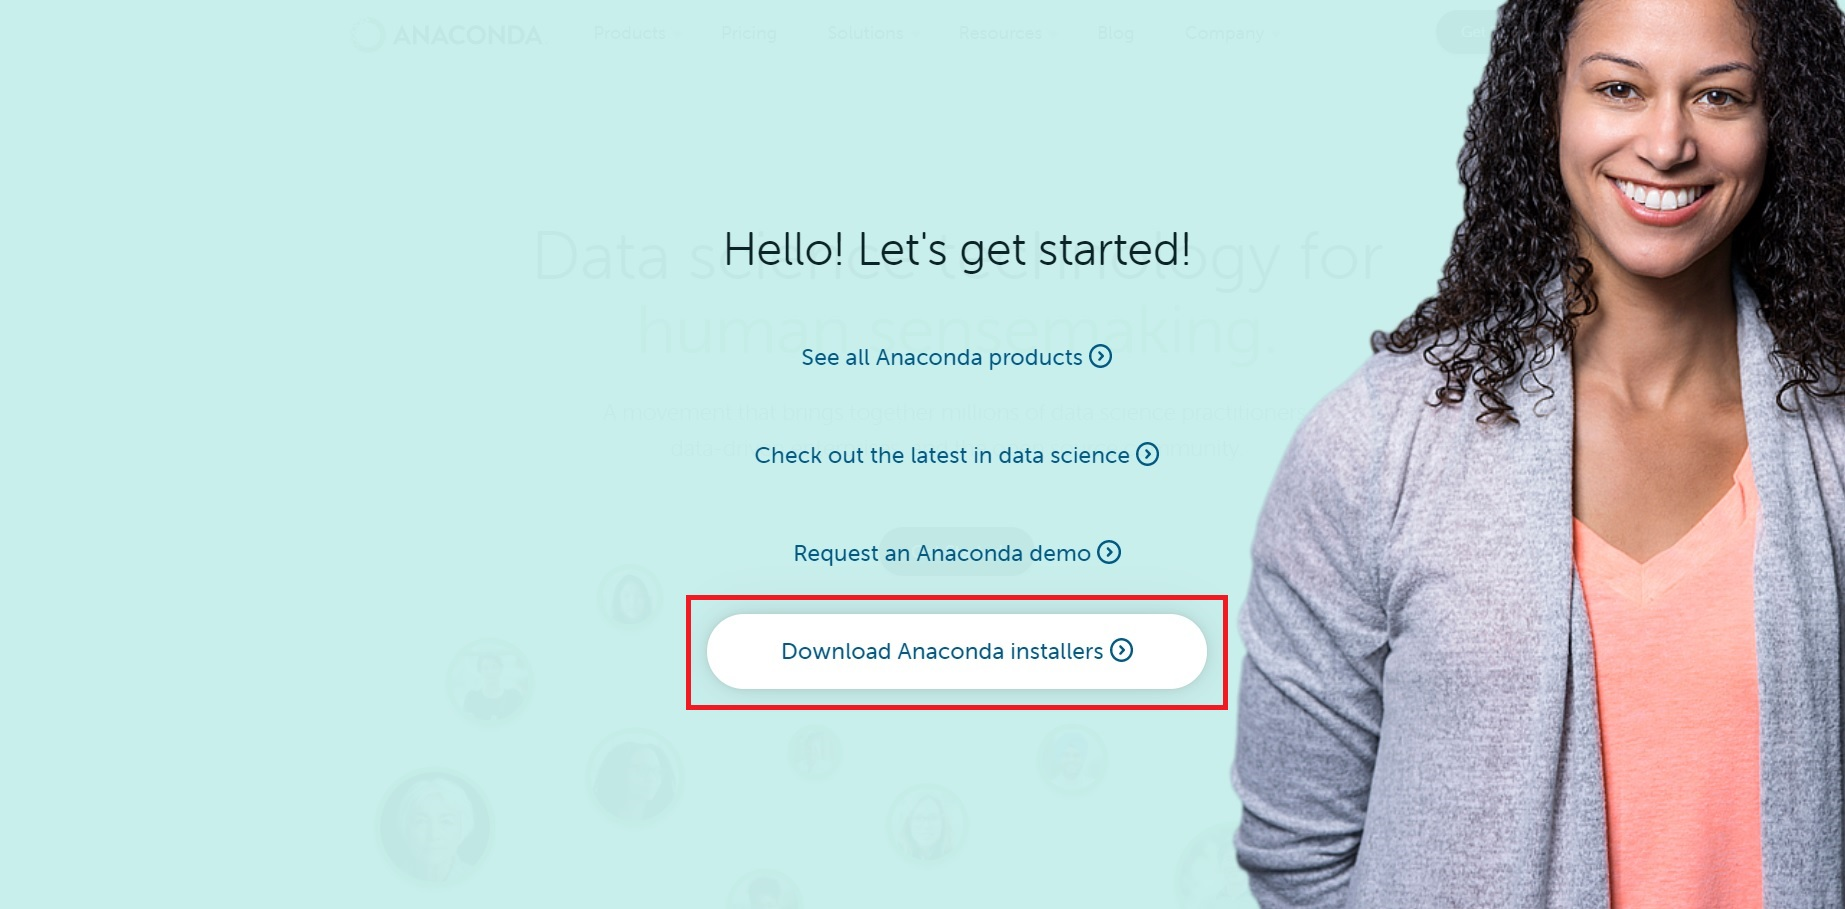
\includegraphics[width=450pt]{./fotos/introduccion/web Anaconda 2.jpg}
\end{center}
\end{figure}

Y seleccionamos la version compatible con nuestro sistema, en este caso Windows 10 de 64 bits:

\begin{figure}[H]
\begin{center}
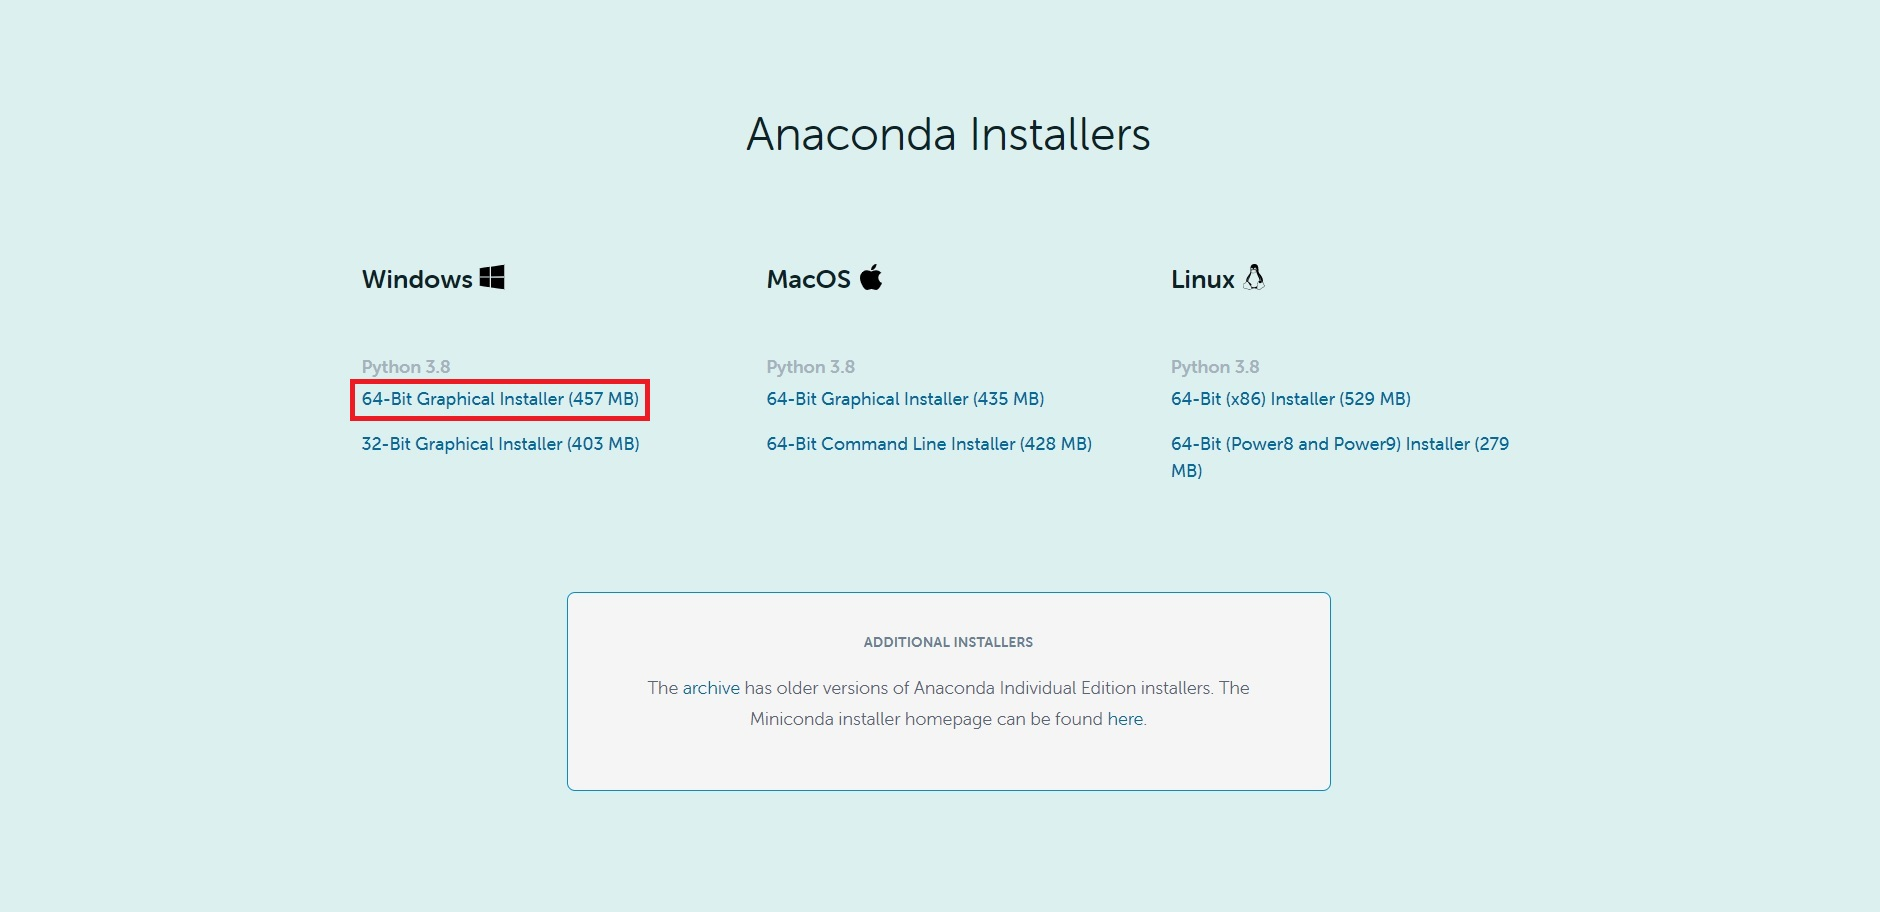
\includegraphics[width=450pt]{./fotos/introduccion/web Anaconda 3.jpg}
\end{center}
\end{figure}

\clearpage

\subsubsection{Instalacion}

Vamos a nuestra carpeta de descargas e iniciamos el instalador. Durante la instalación dejaremos todos los valores por defecto.


\begin{figure}[H]
\begin{center}
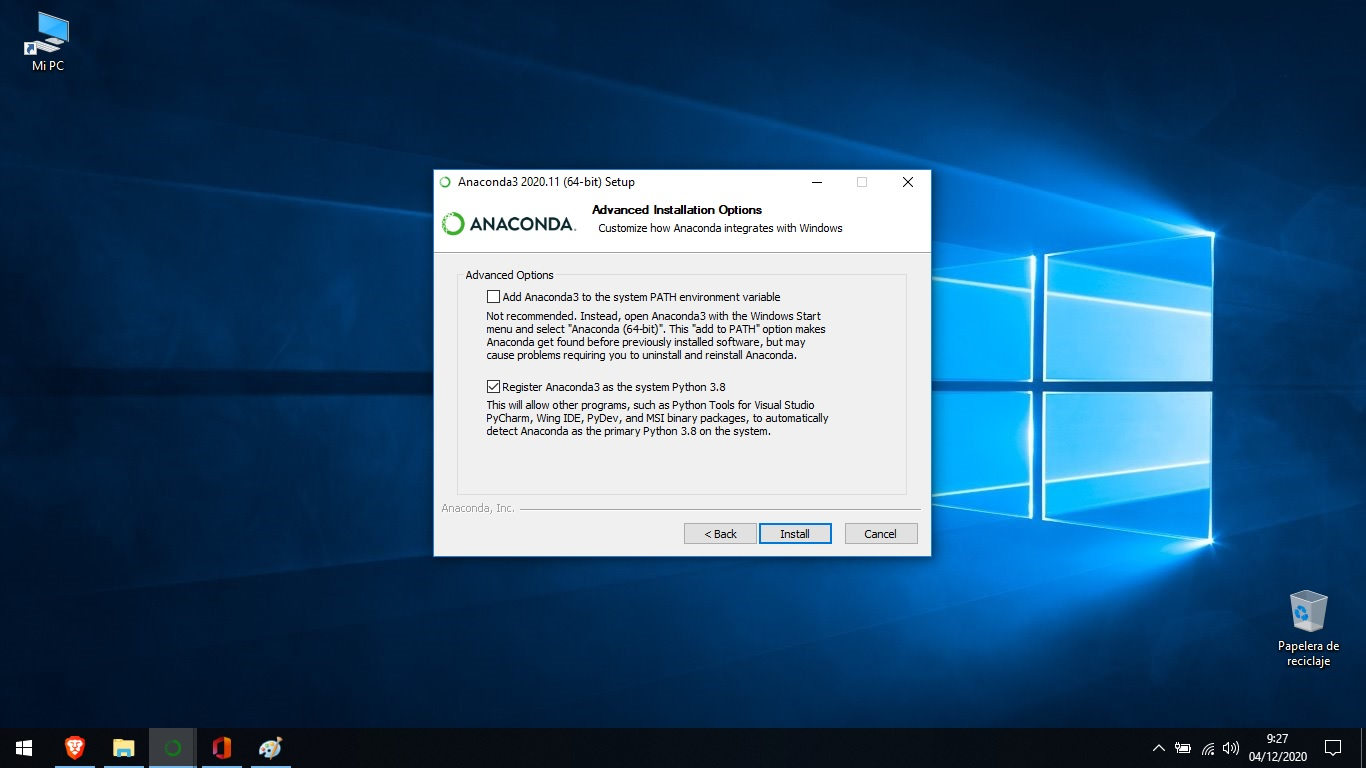
\includegraphics[width=450pt]{./fotos/introduccion/0 - Instalacion Anaconda.jpg}
\end{center}
\end{figure}

Anaconda durante su instalación también nos instalara Python. Para comprobar que ha sido correctamente instalado, vamos a inicio de windows y escribimos \textit{Prompt} y ejecutamos \textit{Anaconda Prompt (Anaconda 3)} como se muestra en la siguiente imagen:

\begin{center}
\begin{figure}[H]
\begin{center}
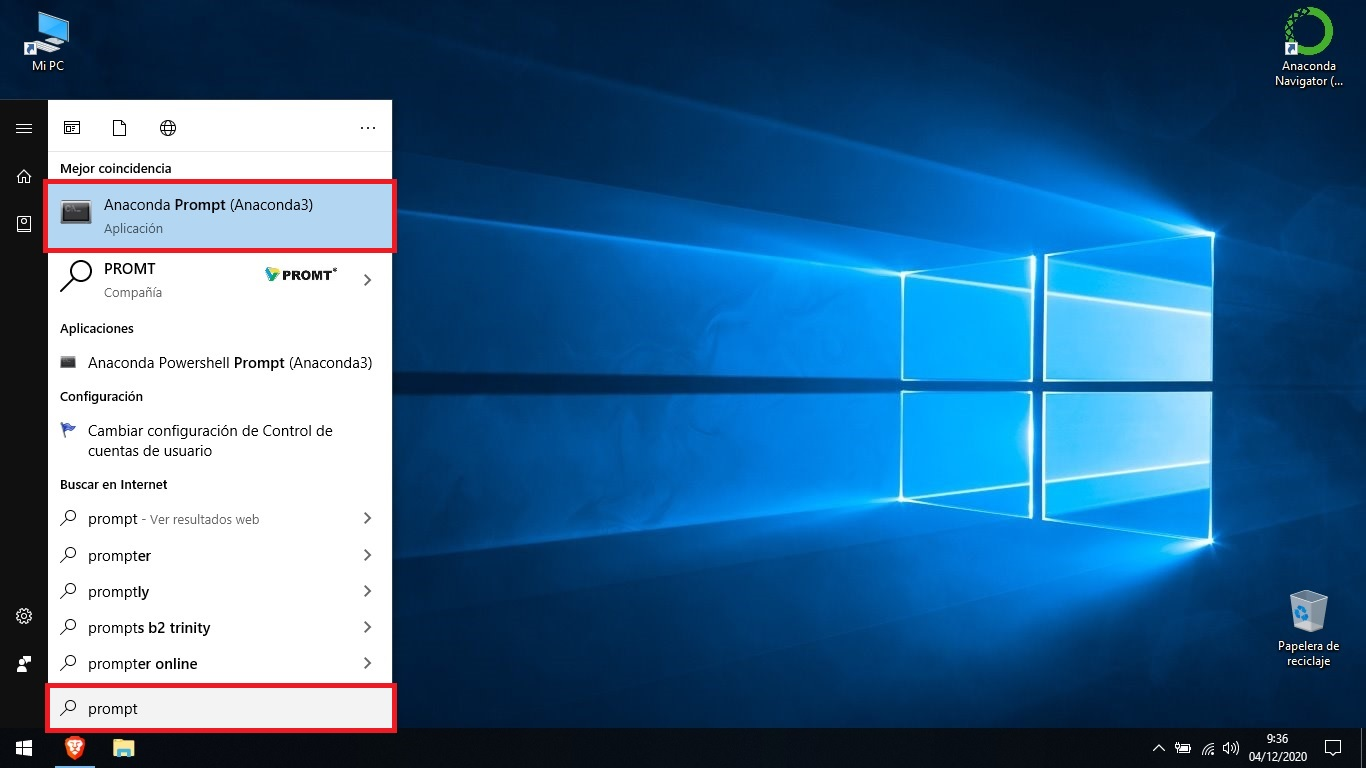
\includegraphics[width=450pt]{./fotos/introduccion/1 - anaconda (V).jpg}
\end{center}
\end{figure}
\vfill
\end{center}

Haremos click derecho y ejecutaremos como administrador. Esto hará que salga una pantalla emergente de windows que nos preguntara si estamos seguros de que queremos permitir que este programa haga modificaciones en el equipo, aceptamos. 

\begin{figure}[H]
\begin{center}
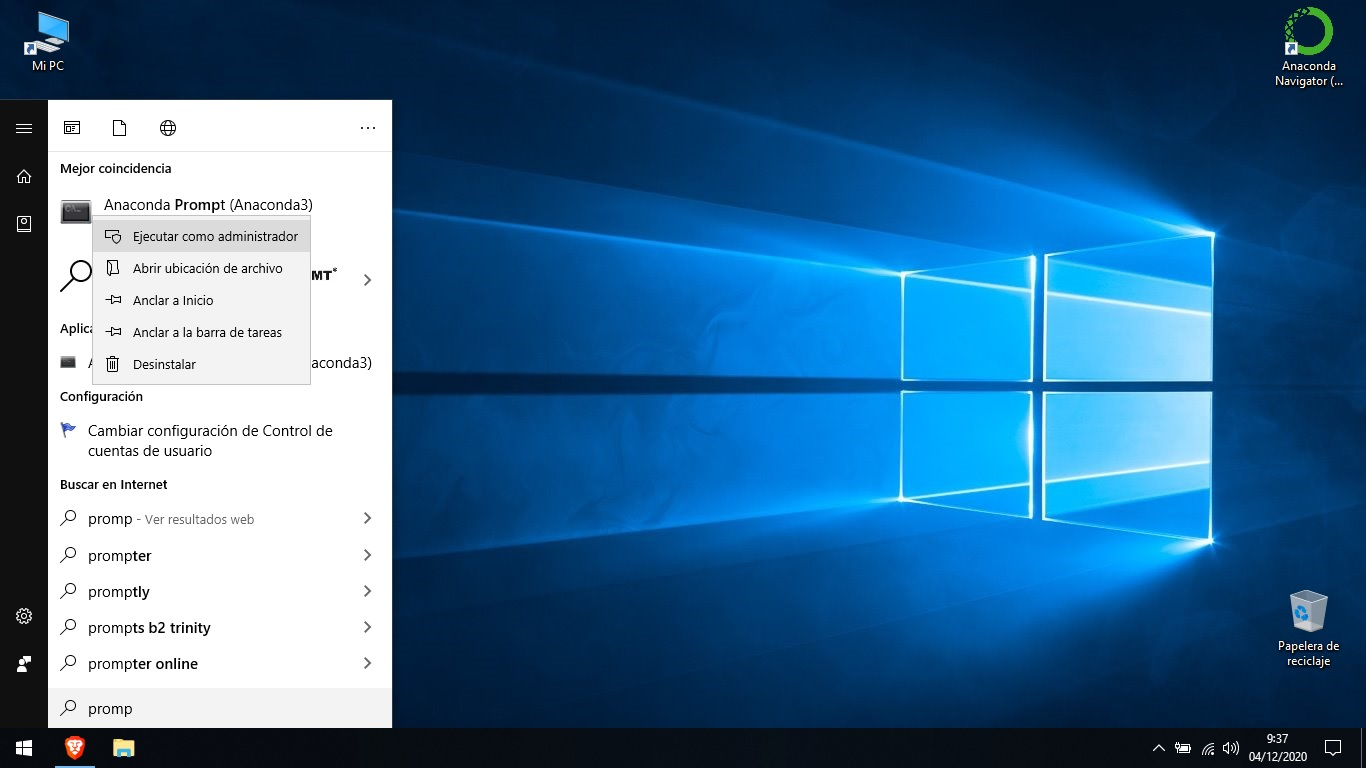
\includegraphics[width=450pt]{./fotos/introduccion/2 - anaconda.jpg}
\end{center}
\end{figure}

NOTA: Si no ejecutamos la consola de Anaconda como administrador, al intentar instalar cualquier librería o paquete extra de python, nos dará error sin especificarnos la razón. Por eso es buena practica acostumbrarse a hacerlo siempre como administrador.

Al ejecutar esta consola veremos que se trata de una similar a la de windows, aunque con la diferencia de que se trata de la propia de Anaconda. Ahora, para asegurarnos de que la instalación de Python ha sido correcta, escribiremos \textbf{python --version}
y si todo ha ido bien obtendremos un mensaje con la version de Python instalado como en la siguiente imagen: 

\begin{figure}[H]
\begin{center}
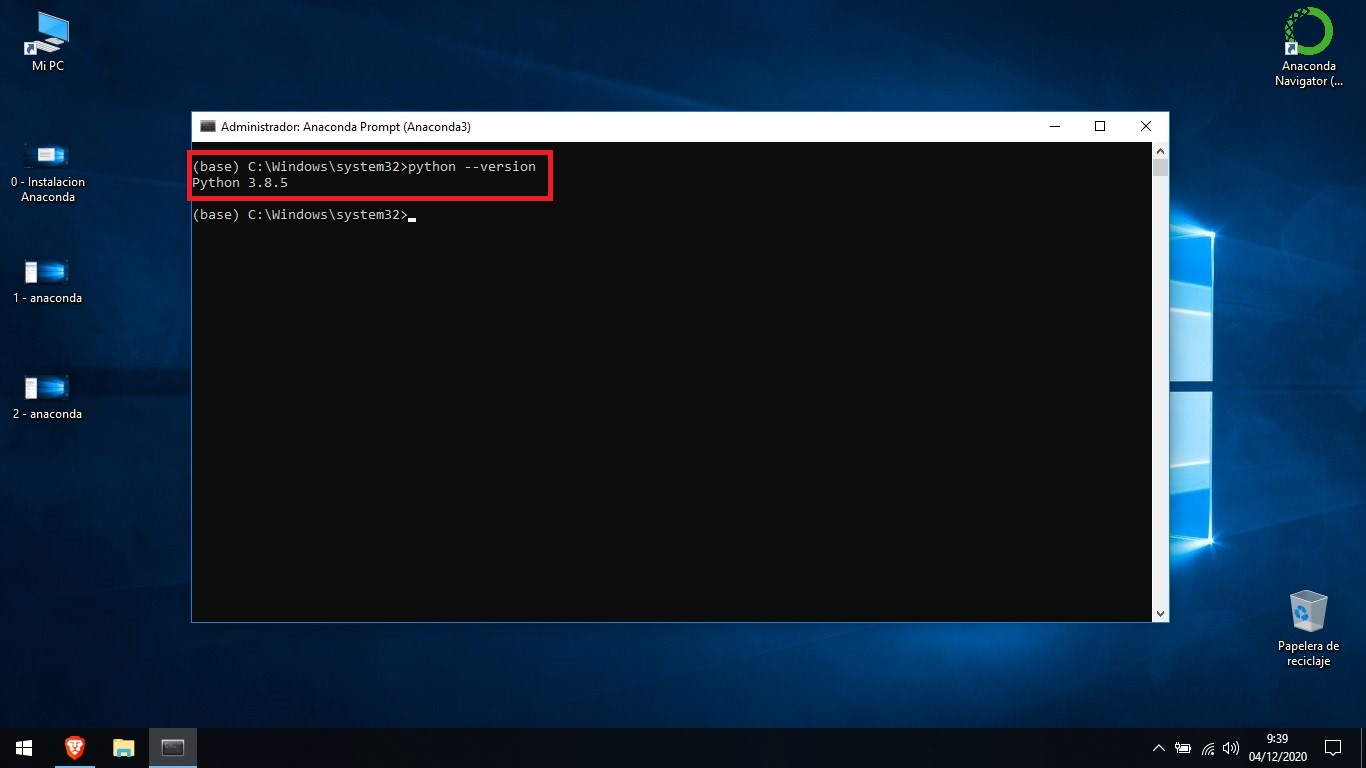
\includegraphics[width=450pt]{./fotos/introduccion/3 - anaconda (V).jpg}
\end{center}
\end{figure}

\subsection{Apache Spark}

\subsubsection{Descarga}

Para instalar Spark vamos a ir a la pagina \href{https://spark.apache.org/}{https://spark.apache.org/}  

Le damos a “Download Spark” 

Y seleccionamos la version que aparece en la foto: 

\begin{figure}[H]
\begin{center}
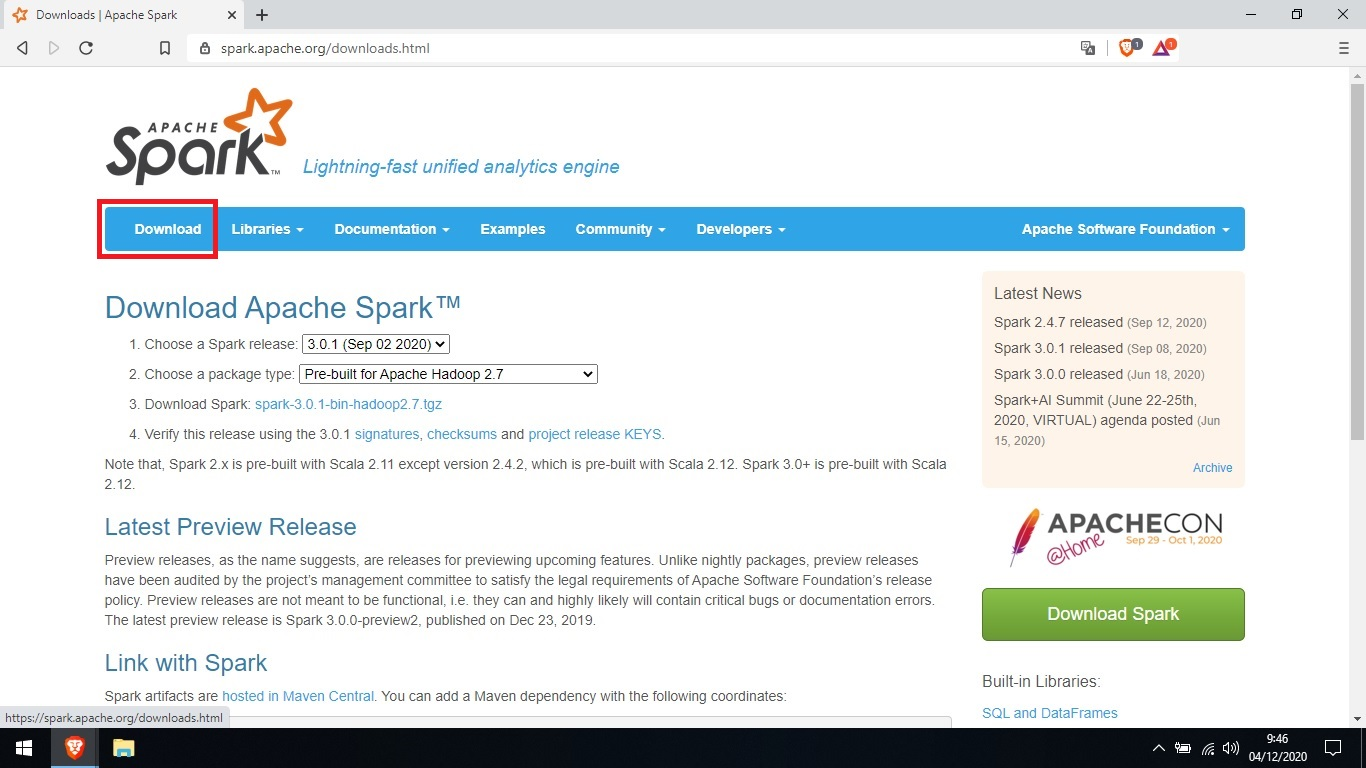
\includegraphics[width=500pt]{./fotos/introduccion/5 - Spark 2 (V).jpg}
\end{center}
\end{figure}

Nos descargara un archivo comprimido con extension “.tgz” 

\begin{figure}[H]
\begin{center}
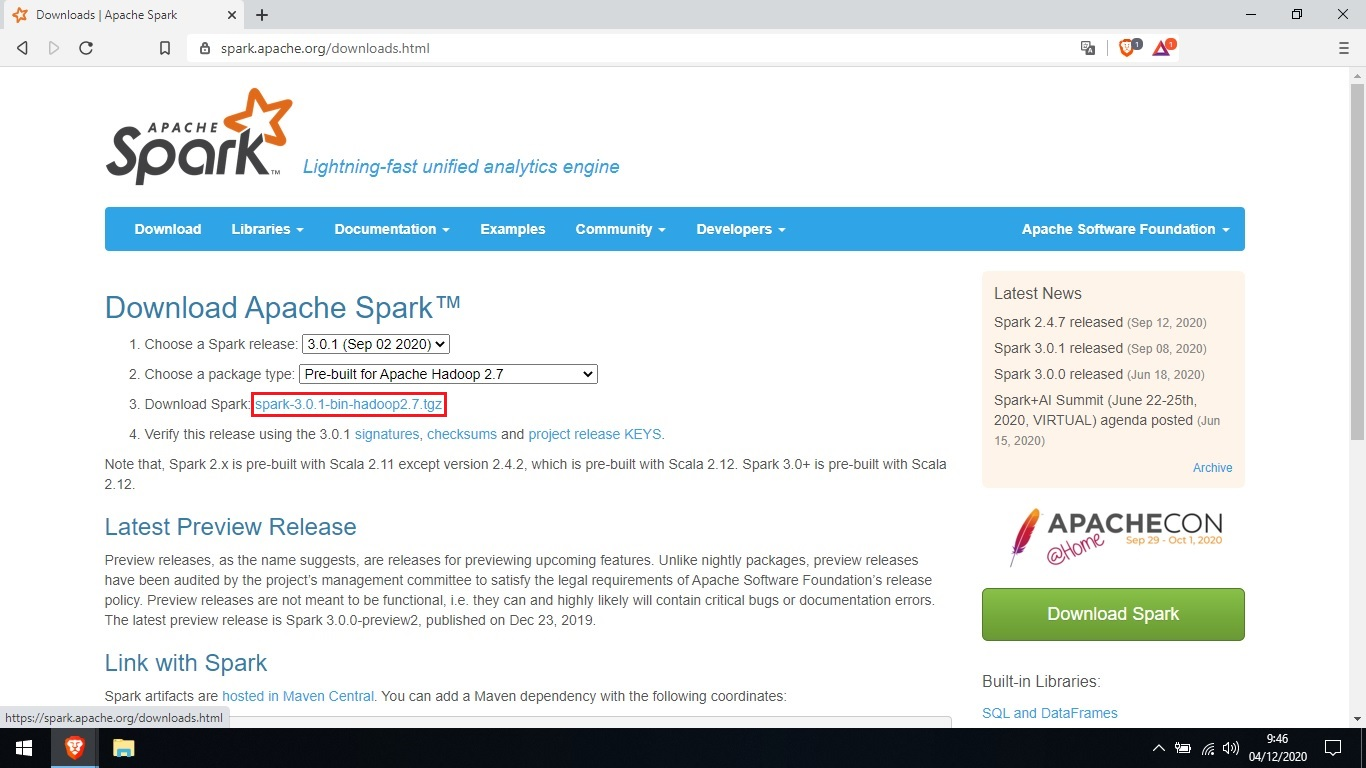
\includegraphics[width=500pt]{./fotos/introduccion/4 - Spark (V).jpg}
\end{center}
\end{figure}

Si ya disponemos de un descompresor instalado lo utilizamos, si no tendremos que descargar uno. En mi caso utilizo 7- Zip por ser software libre. La pagina web es \href{https://www.7-zip.org/}{https://www.7-zip.org/}    

\subsubsection{Instalación}

Ahora igual que tuvimos que hacer con Java JDK, tendremos que crear en la raiz del sistema una carpeta Spark de forma que quede: C:/Spark 

En esta carpeta sera donde descomprimiremos el archivo de Apache Spark recién descargado. Quedara de la siguiente forma: 

\begin{figure}[H]
\begin{center}
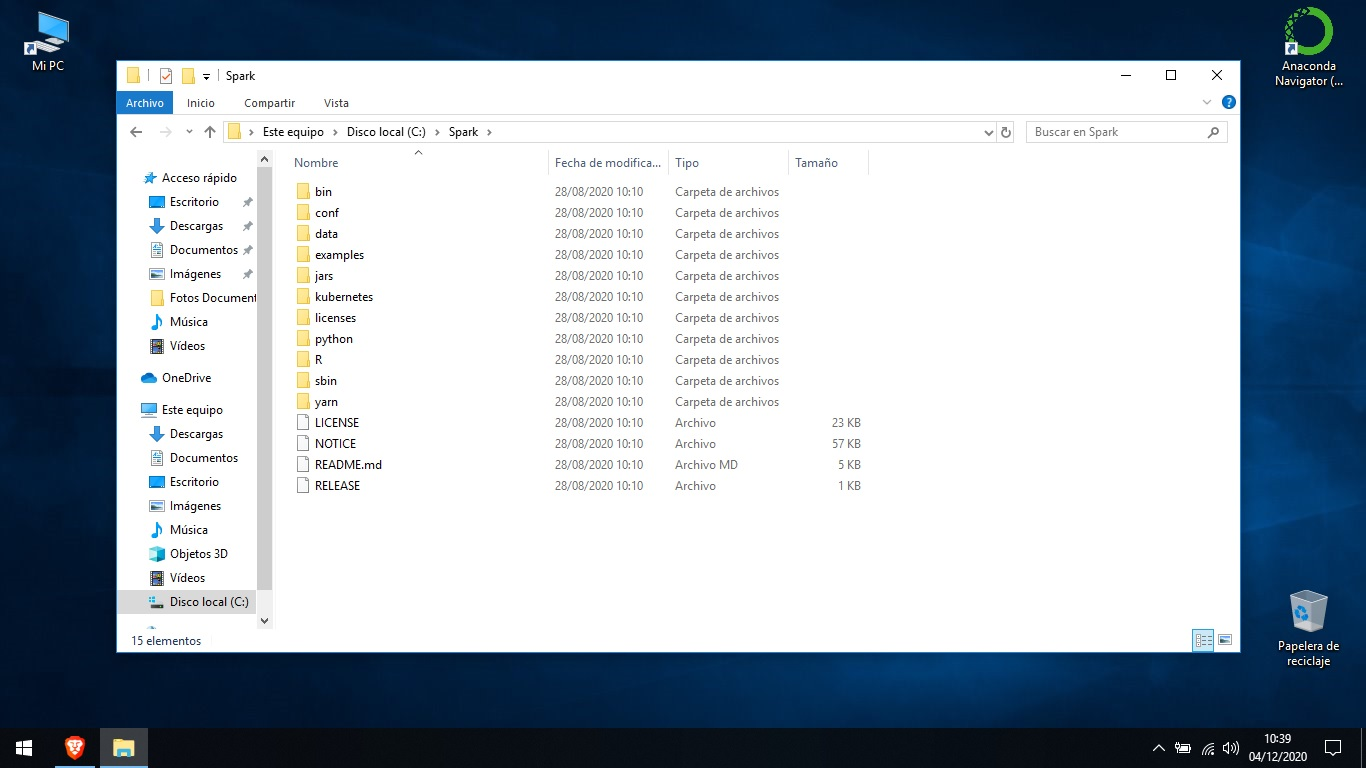
\includegraphics[width=500pt]{./fotos/introduccion/16 - Spark.jpg}
\end{center}
\end{figure}

Ahora algo que también necesitaremos sera Winutils. Antes de que te preguntes qué es eso de Winutils, déjame decirte que son un conjunto de herramientas necesarias para que la instalación de Hadoop pueda funcionar en Windows. 

Si recuerdas, en el momento de la descarga de Apache Spark indicamos que queríamos el paquete con Apache Hadoop 2.7 y una de las condiciones que existen para que Hadoop funcione en ordenadores con Windows es la presencia de Winutils en el directorio bin de su instalación. Esto se indica en la \href{https://cwiki.apache.org/confluence/display/HADOOP2/WindowsProblems}{documentación oficial de Apache Hadoop}.

Una vez descargado el \href{https://github.com/steveloughran/winutils}{repositorio de GitHub} buscamos la carpeta con la versión de las winutils para nuestra versión de Hadoop  y la copiaremos en una carpeta a la que llamarémos hadoop-2.7.1 como hicimos con Spark:

\begin{figure}[H]
\begin{center}
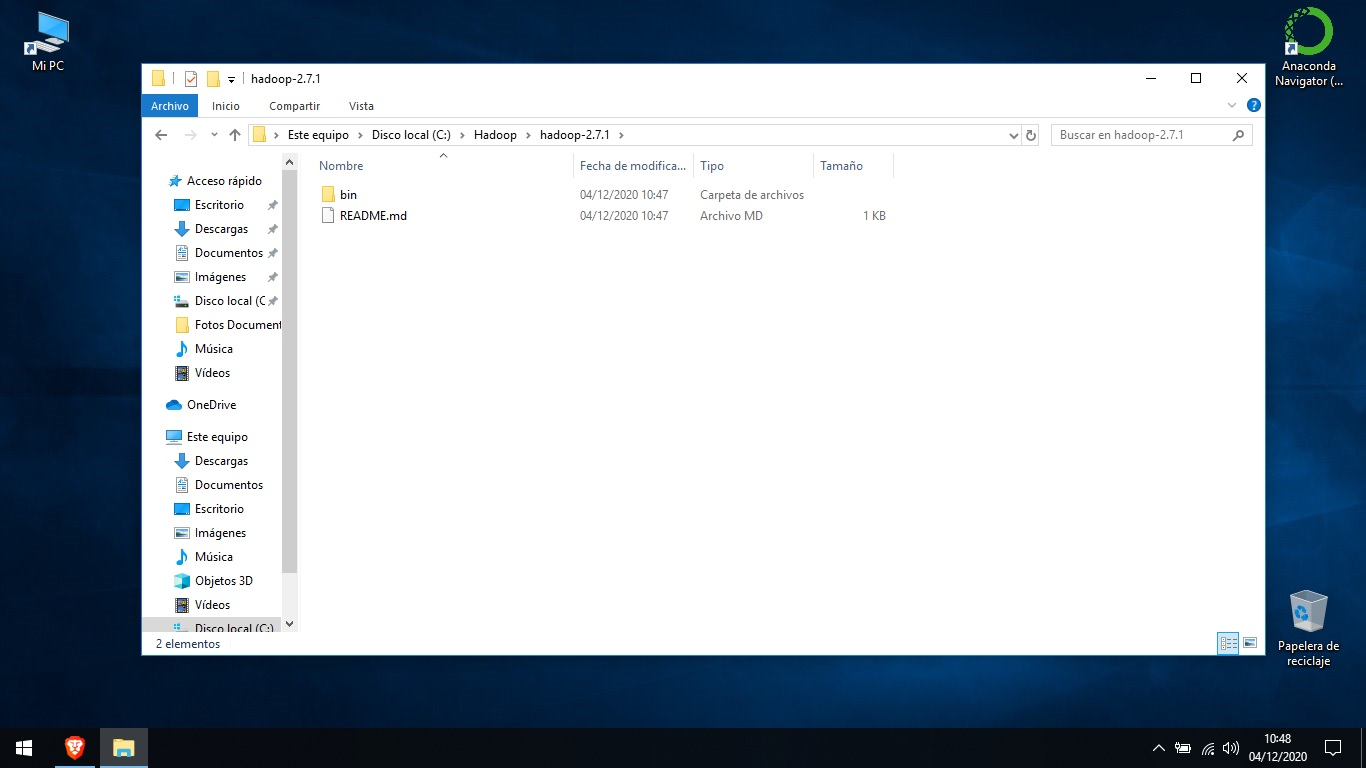
\includegraphics[width=500pt]{./fotos/introduccion/17 - Hadoop.jpg}
\end{center}
\end{figure}

\subsubsection{Variables de entorno}

En concreto vamos a crear tres variables de entorno y modificar la variable Path.

$\bullet$ SPARK\_HOME: Ruta al directorio donde hemos descomprimido el paquete de Apache Spark. 

$\bullet$ HADOOP\_HOME: Apunta al directorio donde hemos copiado la carpeta con el archivo Winutils. 

$\bullet$ JAVA\_HOME: Es el directorio donde se ha instalado el JDK de Java

$\bullet$ PATH: Aquí añadiremos dos nuevas rutas. El directorio bin de la carpeta de Apache Spark y el directorio bin de la carpeta JDK de Java. 

\subsubsection{Scala y Python desde consola}

\subsubsection{Ejecutando Spark-shell y pyspark desde consola}

\begin{figure}[H]
\begin{center}
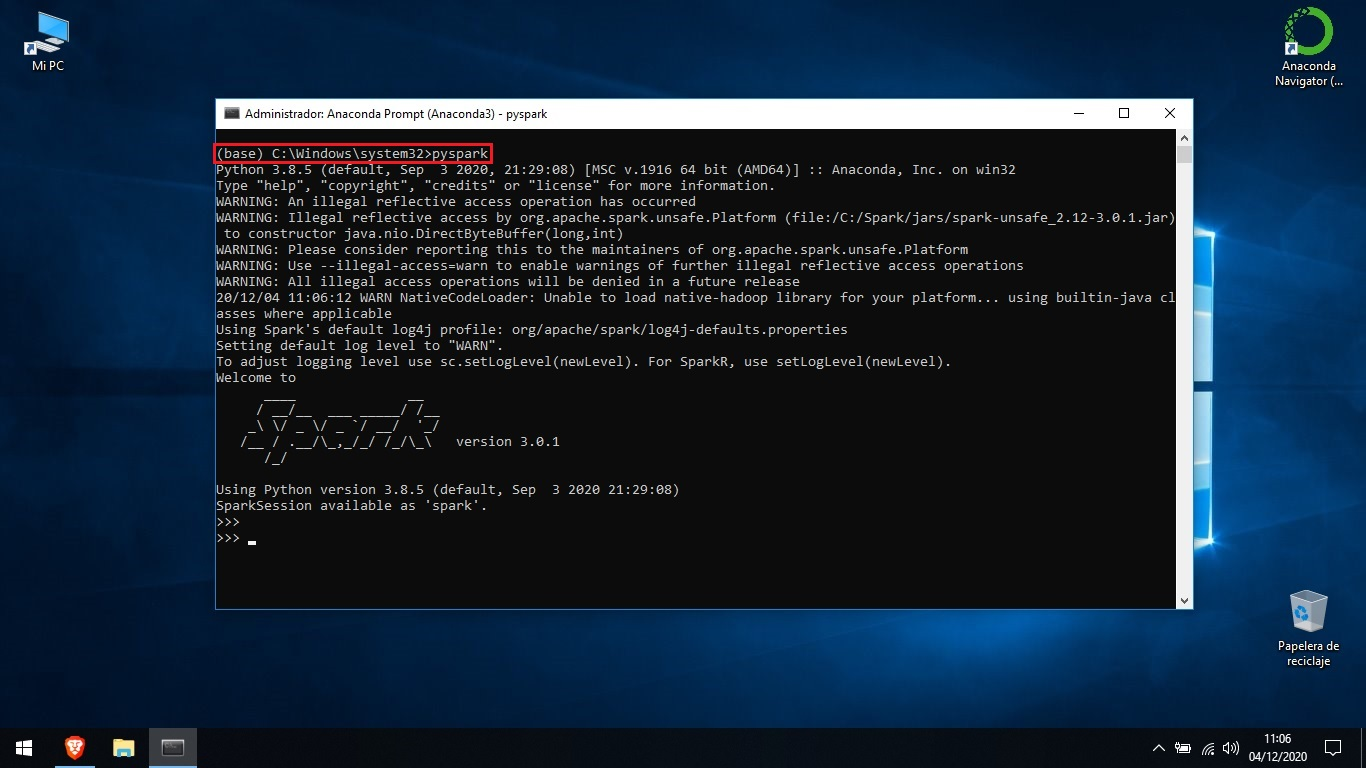
\includegraphics[width=500pt]{./fotos/introduccion/18 - Pyspark funcionando (V).jpg}
\end{center}
\end{figure}

\begin{figure}[H]
\begin{center}
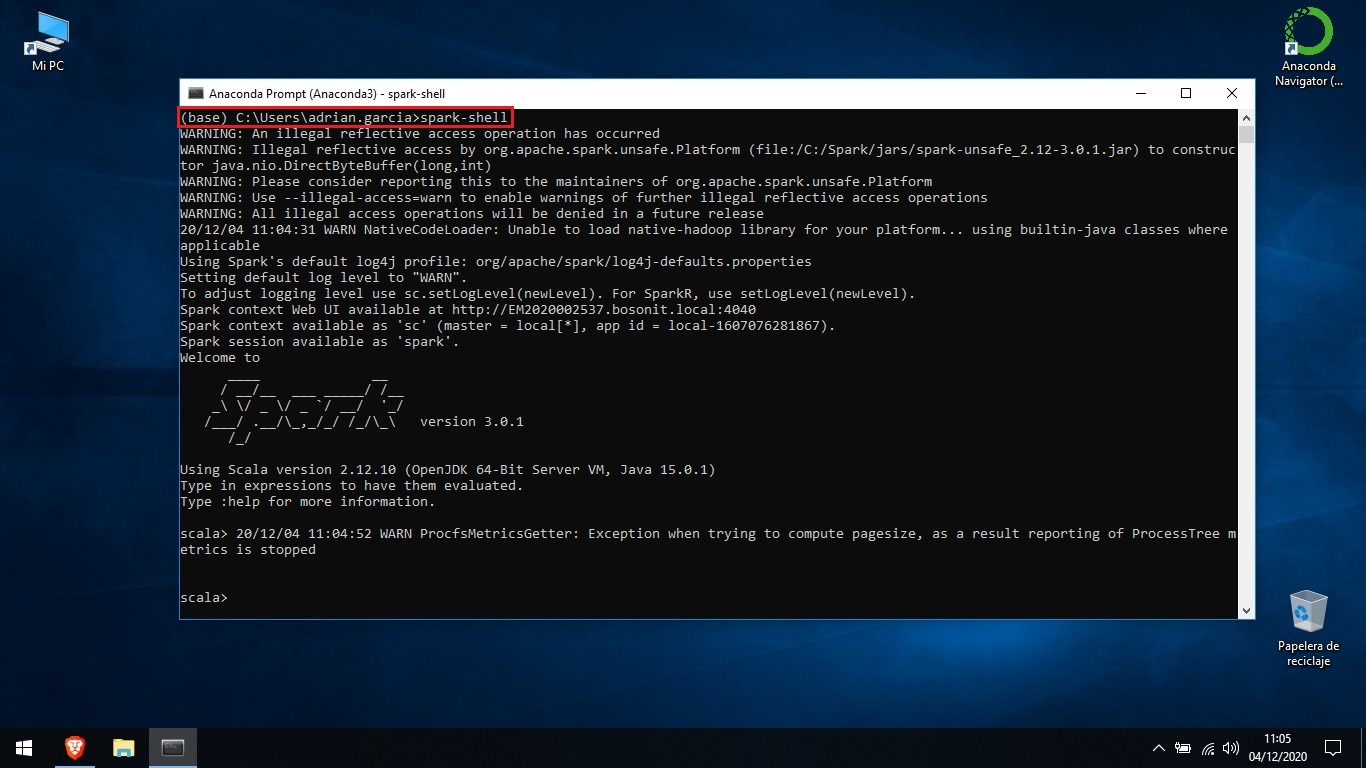
\includegraphics[width=500pt]{./fotos/introduccion/18 - Scala funcionando (V).jpg}
\end{center}
\end{figure}

Ejecutar en la consola de anaconda pip install pyspark 

\subsubsection{Jupyter Notebook desde consola con Pyspark}

Añadimos las variables de entorno de jupyter y notebook 

\begin{figure}[H]
\begin{center}
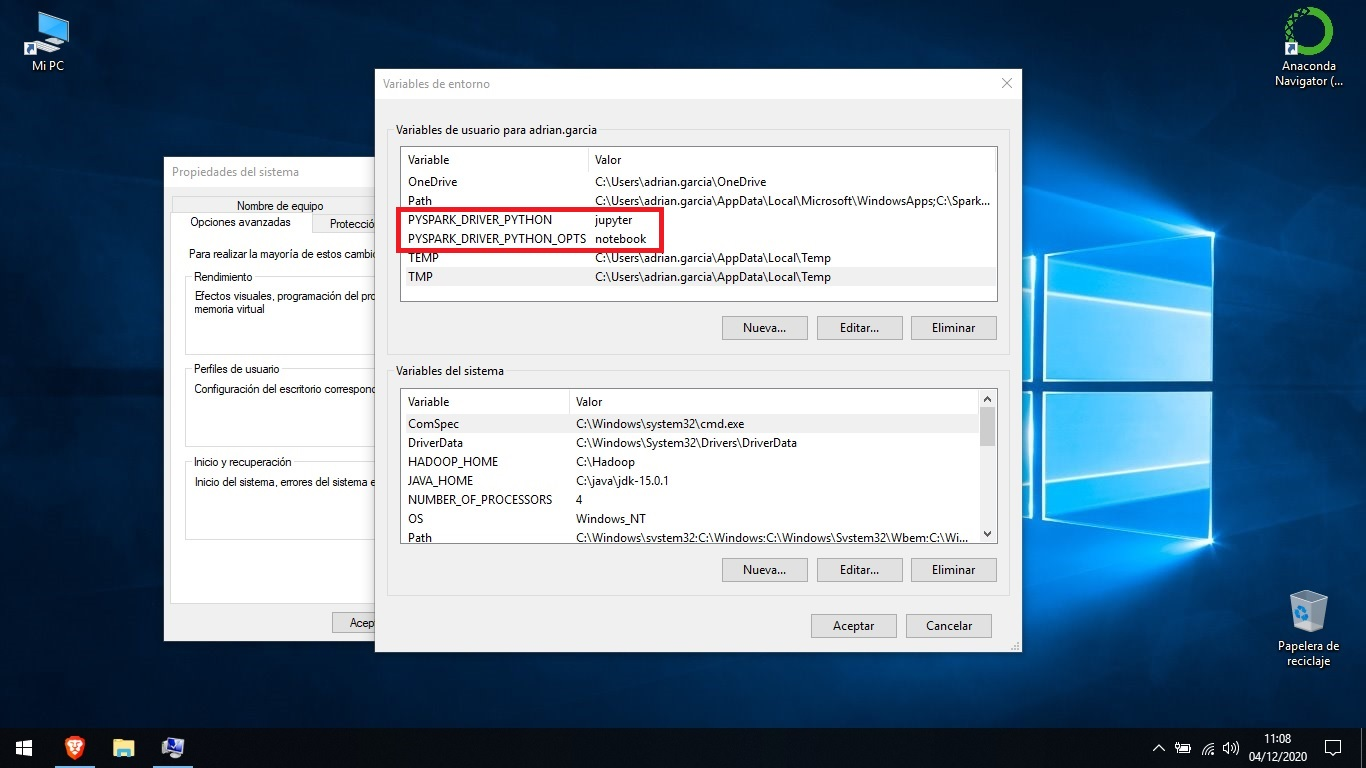
\includegraphics[width=500pt]{./fotos/introduccion/19 - notebook desde comandos (V).jpg}
\end{center}
\end{figure}

Hacemos pyspark en la consola de anaconda. Nos abrirá un notebook y en la consola veremos:

\begin{figure}[H]
\begin{center}
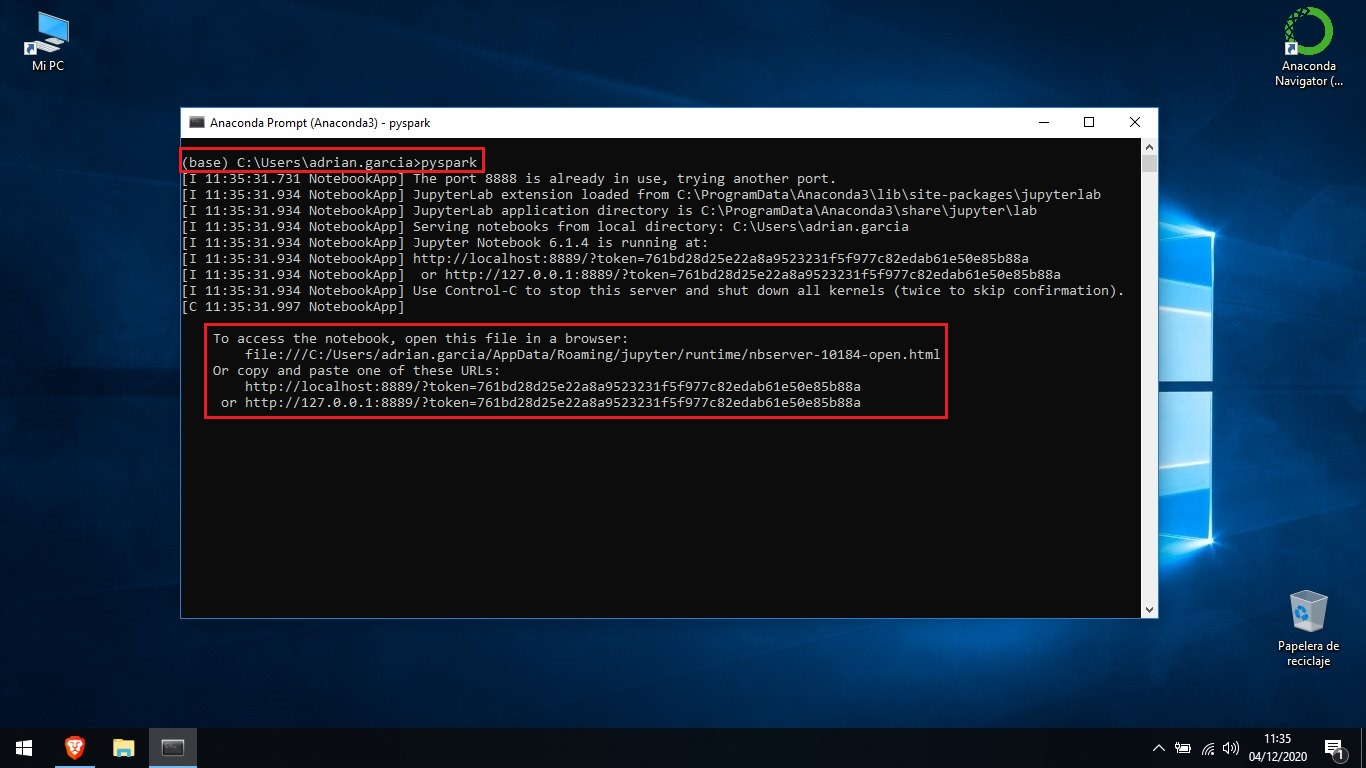
\includegraphics[width=500pt]{./fotos/introduccion/21 - Abriendo notebook al ejecutar pyspark (V).jpg}
\end{center}
\end{figure}

\subsubsection{Pyspark en anaconda}

\begin{figure}[H]
\begin{center}
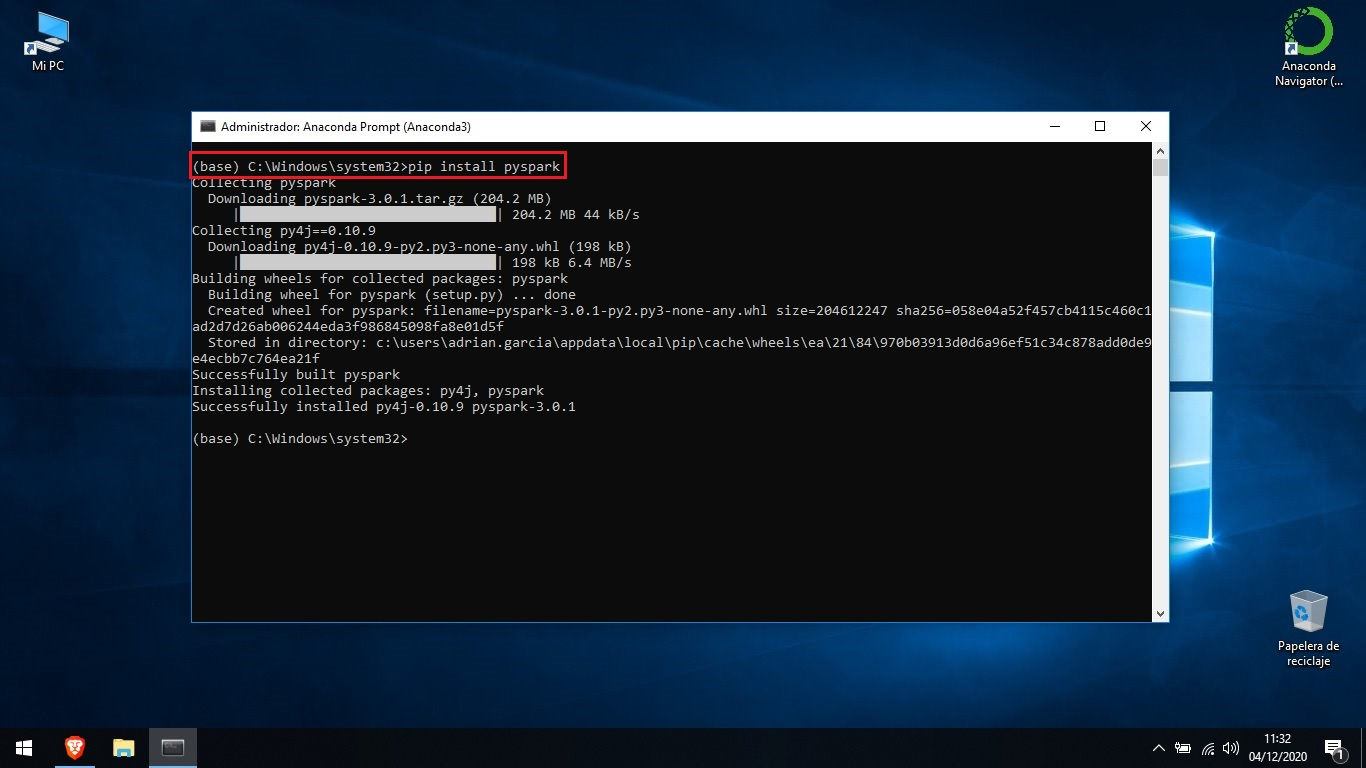
\includegraphics[width=500pt]{./fotos/introduccion/20 - instalando pyspark anaconda (V).jpg}
\end{center}
\end{figure}

\subsubsection{Scala desde Jupyter Notebook}

Abrimos la consola de anaconda 

Ejecutamos el siguiente codigo que instalara el interprete de Scala:

\lstset{language=bash, breaklines=true, basicstyle=\ttfamily}
\begin{lstlisting}[frame=single]
pip install spylon-kernel 
\end{lstlisting}

Añadimos que nos permita seleccionar el kernel de scala desde el notebook. Para ello ejecutamos

\lstset{language=bash, breaklines=true, basicstyle=\ttfamily}
\begin{lstlisting}[frame=single]
python -m spylon\_kernel install
\end{lstlisting}


En CentOS:

\lstset{language=bash, breaklines=true, basicstyle=\ttfamily}
\begin{lstlisting}[frame=single]
python -m spylon_kernel install --user
\end{lstlisting}

Ahora si abrimos un notebook desde anaconda veremos como se indica en la foto que nos da la opción de crear un notebook de Scala: 

\begin{figure}[H]
\begin{center}
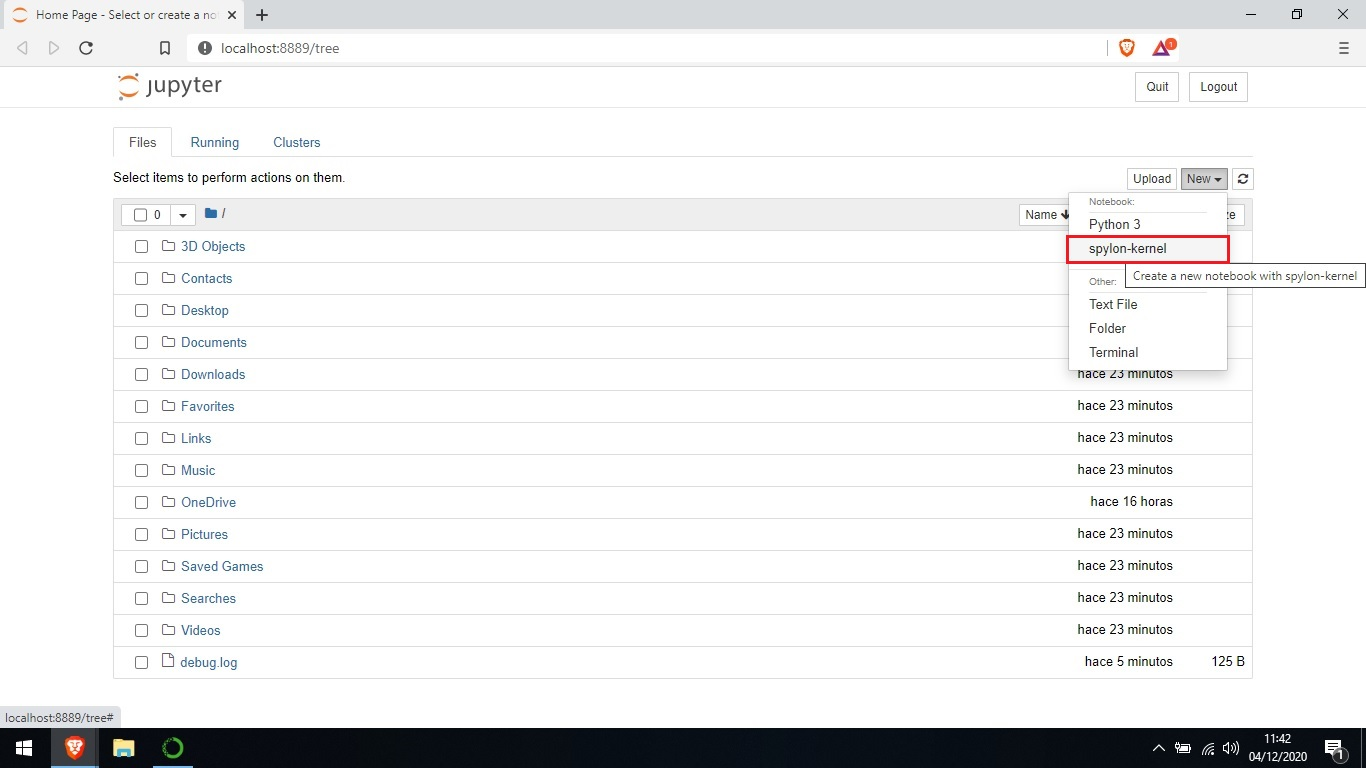
\includegraphics[width=450pt]{./fotos/introduccion/22 - Scala desde notebook de anaconda (V).jpg}
\end{center}
\end{figure}

Y podemos verlo en funcionamiento:

\begin{figure}[H]
\begin{center}
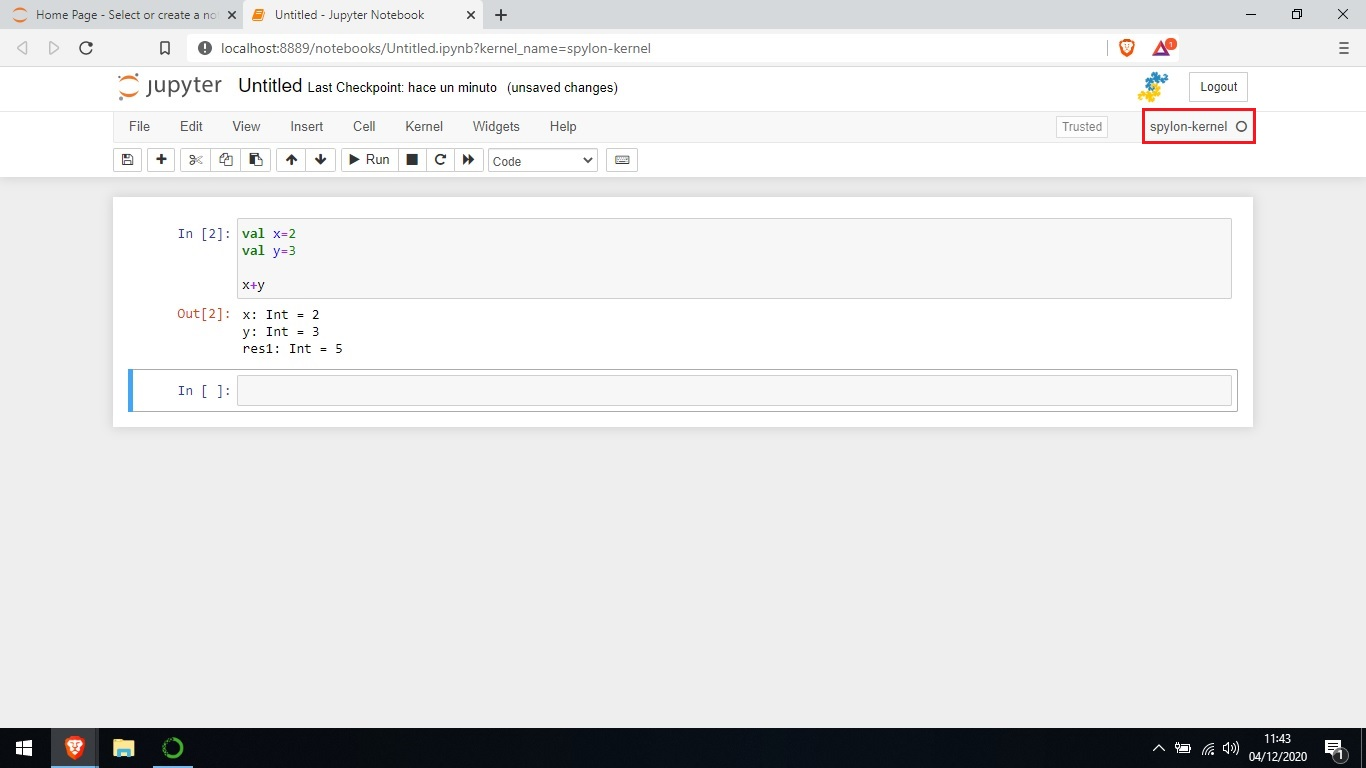
\includegraphics[width=450pt]{./fotos/introduccion/23 - Scala en notebook funcionando (V).jpg}
\end{center}
\end{figure}

\subsubsection{R desde Jupyter Notebook}

Podemos añadir el lenguaje R a nuestro Jupyter Notebook ejecutando el siguiente comando en Anaconda Prompt:

\lstset{language=bash, breaklines=true, basicstyle=\ttfamily}
\begin{lstlisting}[frame=single]
conda install -c r r-irkernel
\end{lstlisting}

\clearpage

\subsection{Apache Kafka}

\subsubsection{Descarga}

Para instalar Apache Kafka vamos a ir a su web oficial:

\begin{center}
\href{https://kafka.apache.org/}{https://kafka.apache.org/}  
\end{center}

Le damos a “DOWNLOAD KAFA” en la parte superior derecha como se puede ver en la siguiente imagen: 

\begin{figure}[H]
\begin{center}
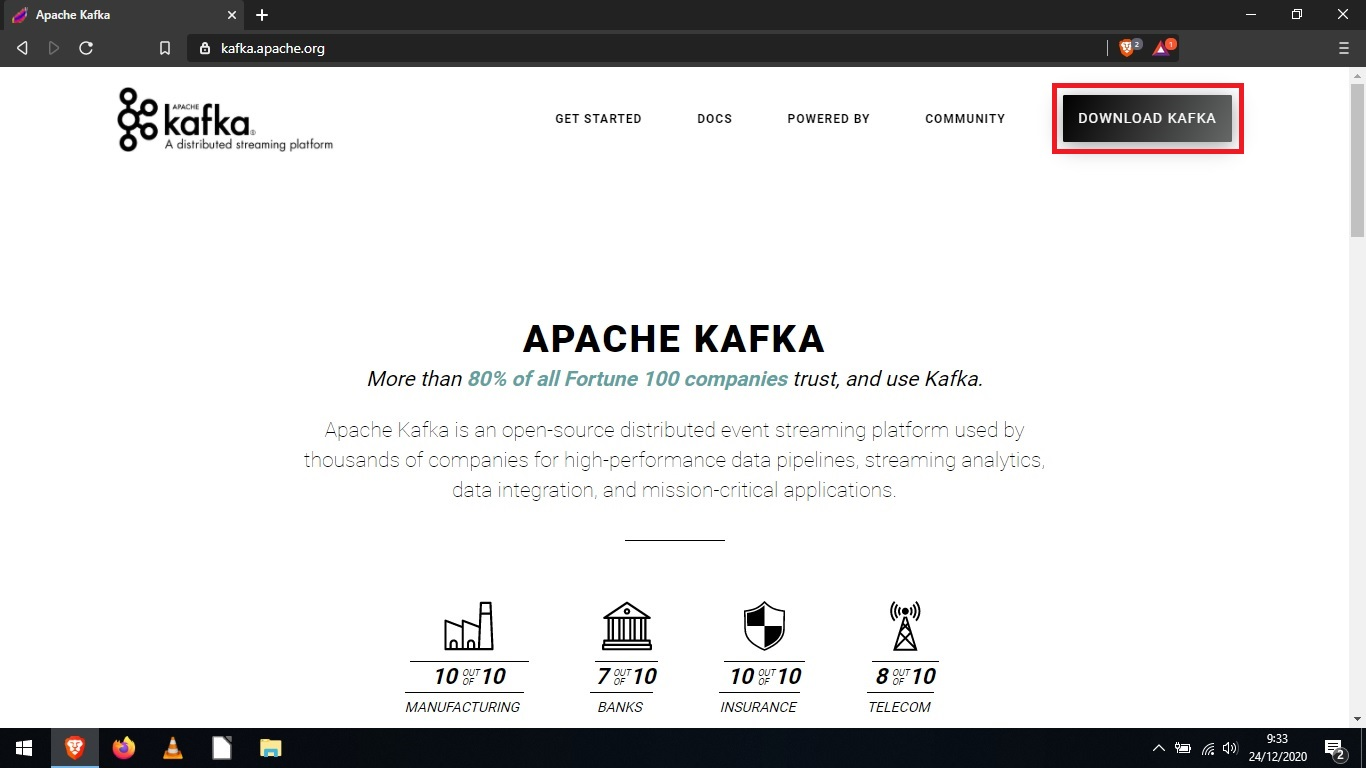
\includegraphics[width=450pt]{./fotos/Kafka/01 (V).jpg}
\end{center}
\end{figure}

Y descargamos el archivo tgz haciendo click en el nombre del archivo: 

\begin{figure}[H]
\begin{center}
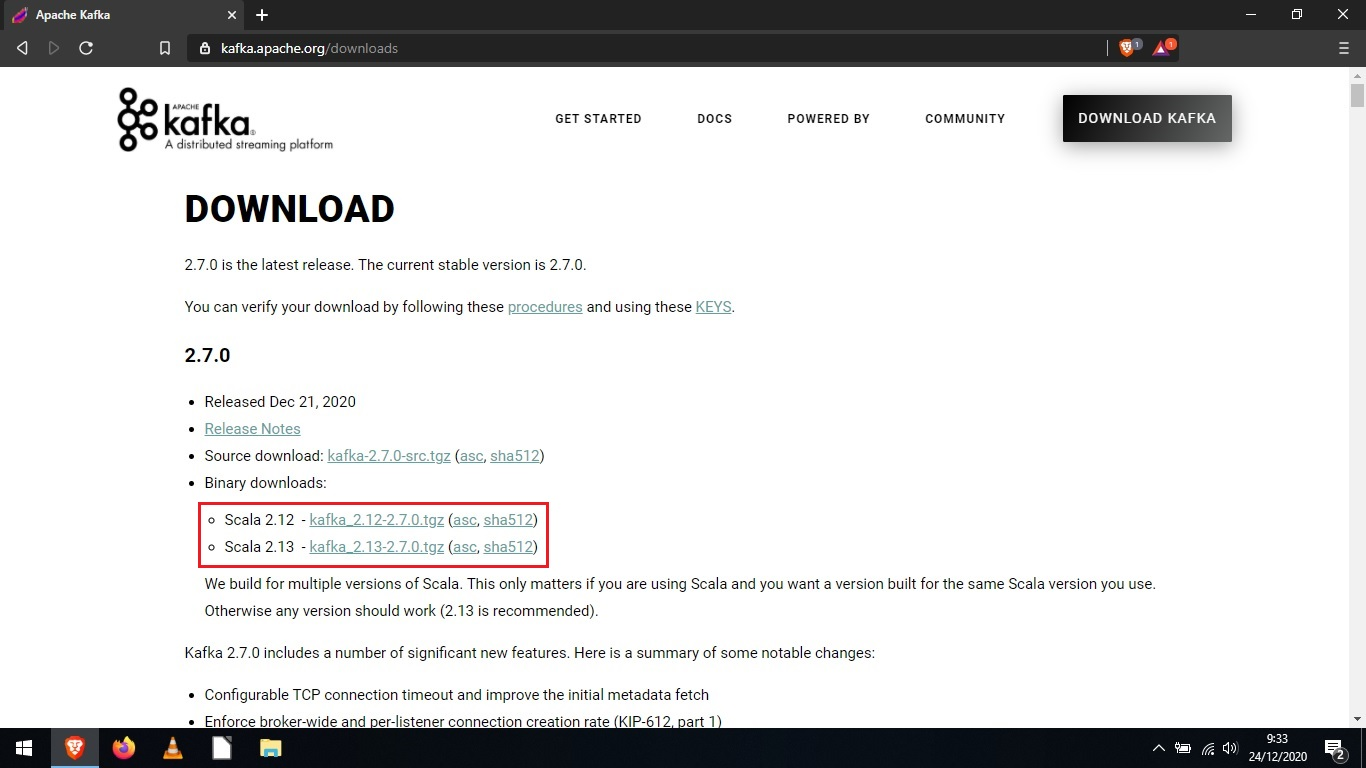
\includegraphics[width=450pt]{./fotos/Kafka/02 (V).jpg}
\end{center}
\end{figure} 

\subsubsection{Instalación}

De la misma forma que con Java o Spark, tendremos que crear en la raiz del sistema una carpeta Kafka de forma que quede: C:/Kafka

Realmente he elegido el nombre Kafka para la carpeta por facilitar el enrutamiento, pero realmente el nombre daria igual siempre y cuando la configuremos bien en las variables de entorno. 

En esta carpeta sera donde descomprimiremos el archivo de Apache Kafka recién descargado. Quedara de la siguiente forma: 

\begin{figure}[H]
\begin{center}
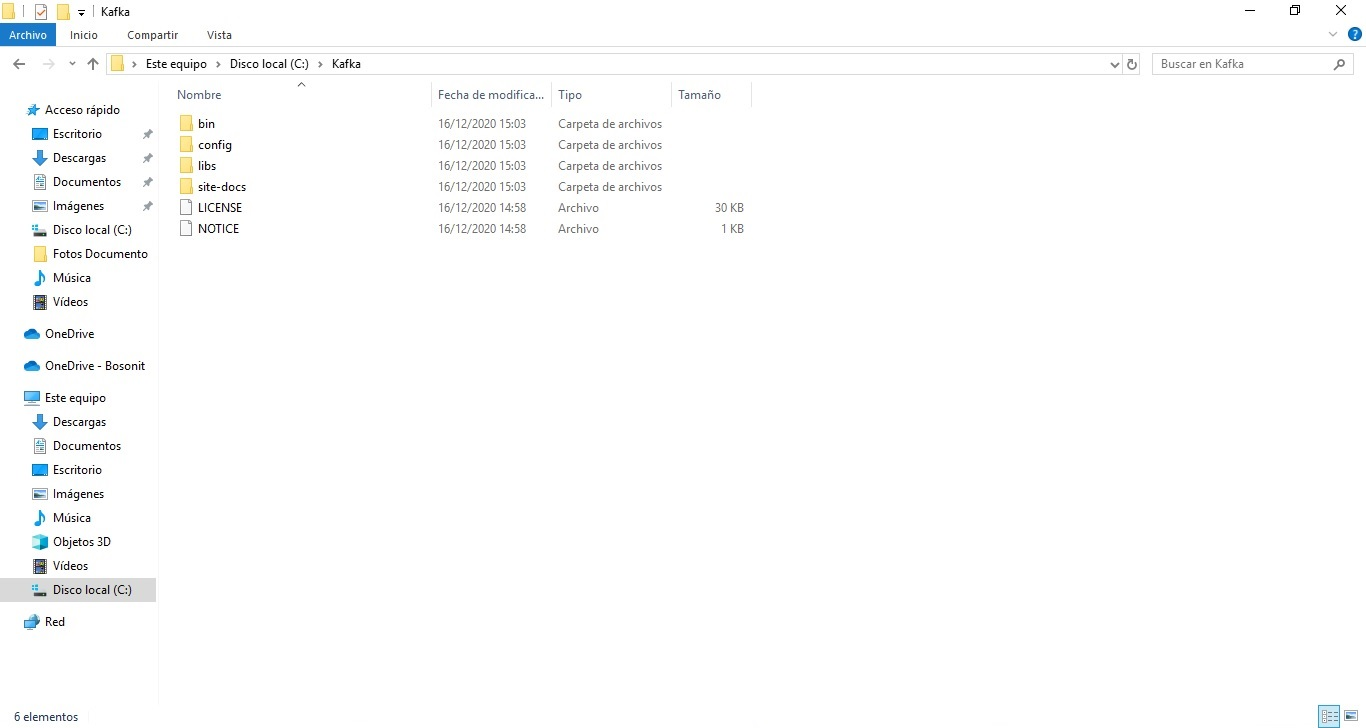
\includegraphics[width=450pt]{./fotos/Kafka/03 (V).jpg}
\end{center}
\end{figure}

\subsubsection{Variables de entorno}

Repetiremos los mismos pasos que en los casos anteriores. De todas formas repetiramos los pasos que hay que seguir. Hacemos click en inicio y escribiremos 'Editar las variables de entorno del sistema' como en la siguiente imagen:

\begin{figure}[H]
\begin{center}
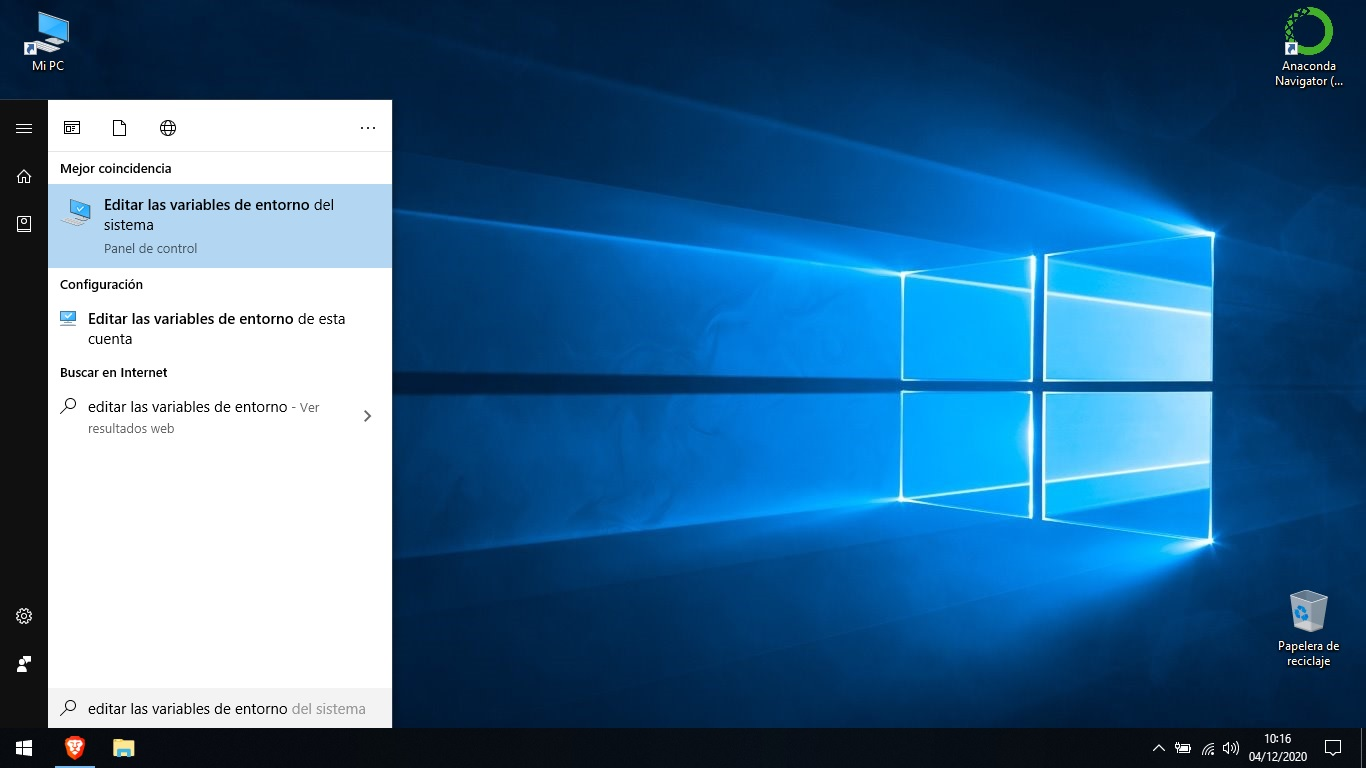
\includegraphics[width=425pt]{./fotos/introduccion/7 - Java.jpg}
\end{center}
\end{figure}

\clearpage

Al abrir el editor veremos que se abre la ventana de Propiedades del sistema. Hacemos click en la pestaña de 'Opciones avanzadas' y abajo hacemos click en 'Variables de entorno':

\begin{figure}[H]
\begin{center}
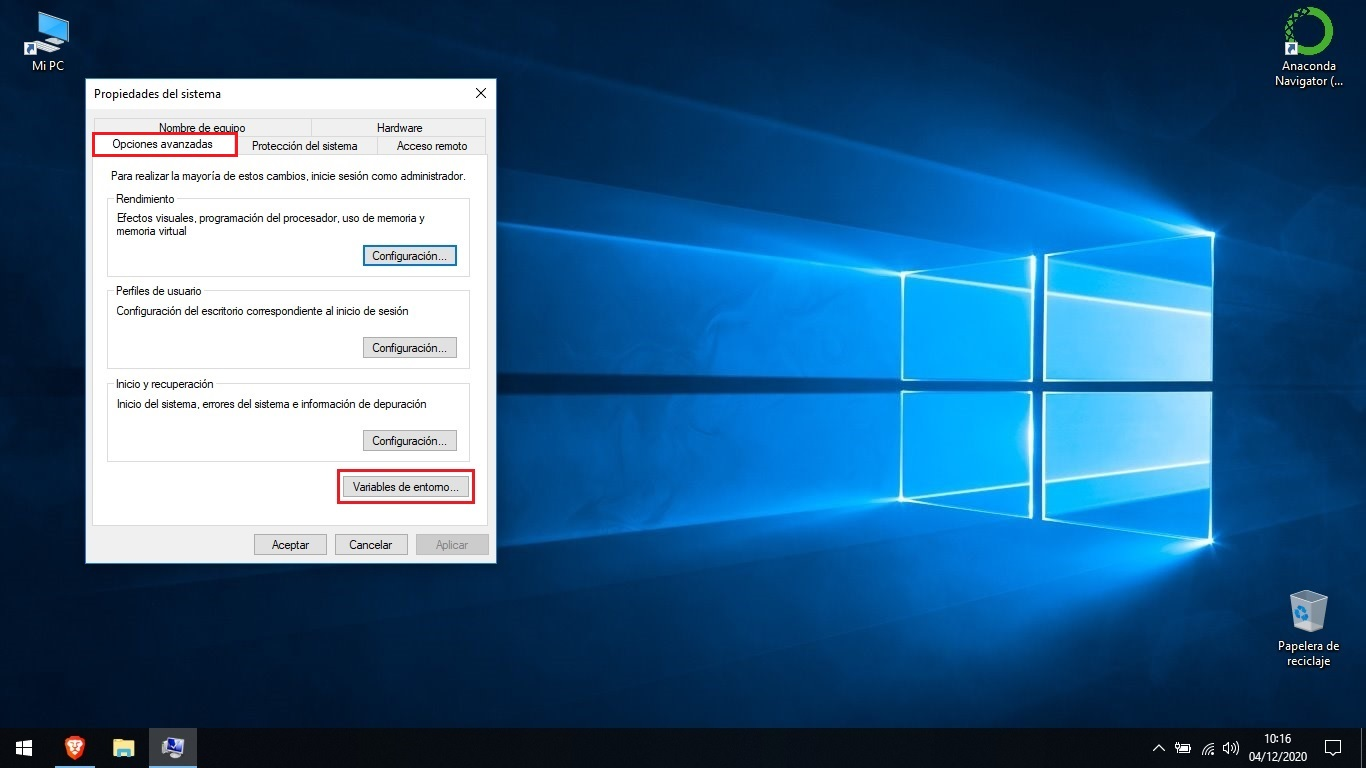
\includegraphics[width=425pt]{./fotos/introduccion/8 - Java (V).jpg}
\end{center}
\end{figure}

En la ventana que se nos ha abierto veremos dos recuadros. En uno pondrá \textit{Variables de usuario} y en el de debajo \textit{Variables del sistema}. Lo mas recomendable es crear las variables de entorno para el sistema, con el fin de que cualquier usuario tenga acceso. 

Entonces en el grupo de Variables del sistema hacemos click en el botón 'Nueva'.

\begin{figure}[H]
\begin{center}
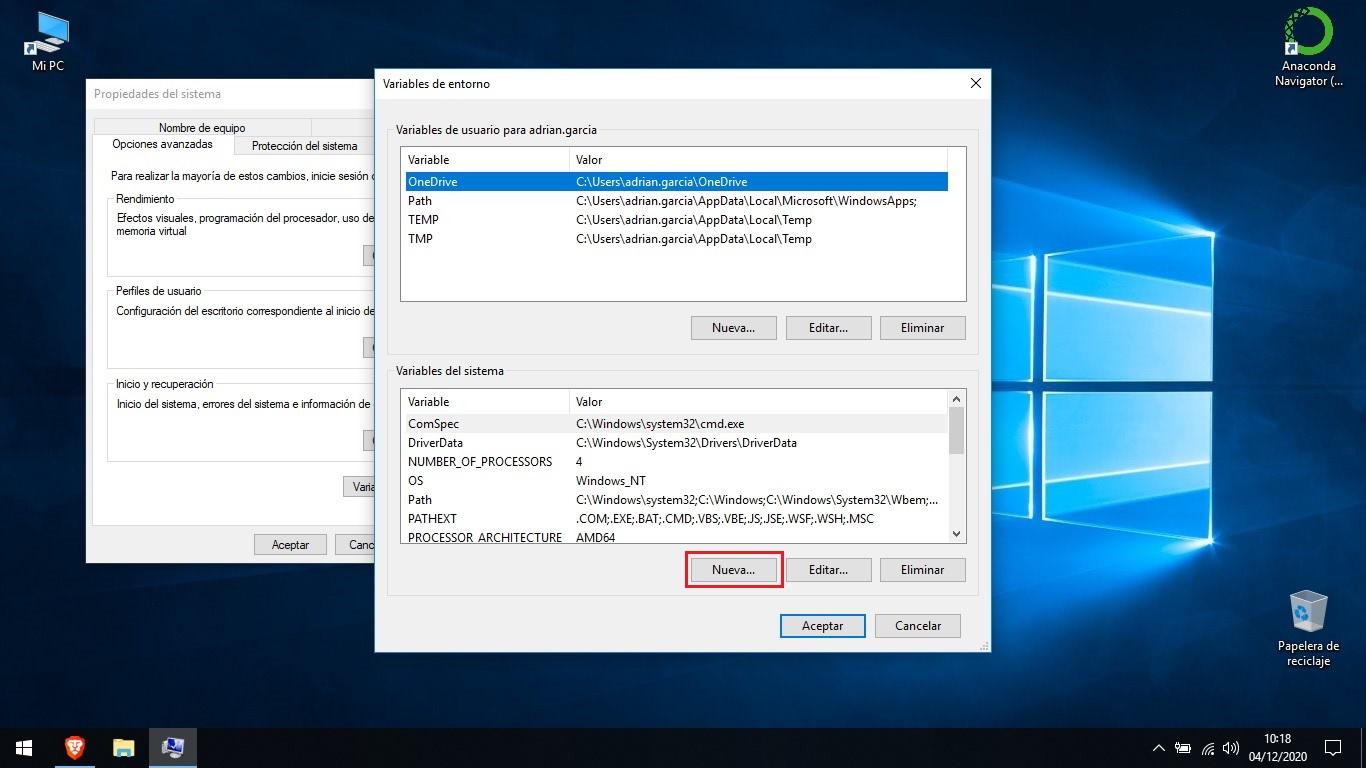
\includegraphics[width=450pt]{./fotos/introduccion/9 - Java (V).jpg}
\end{center}
\end{figure}

\clearpage

En el nombre escribiremos 'KAFKA\_HOME', mientras que en valor la variable escribiremos la ruta donde instalamos Apache Kafka, en nuestro caso será \textit{C:/Kafka}

\begin{figure}[H]
\begin{center}
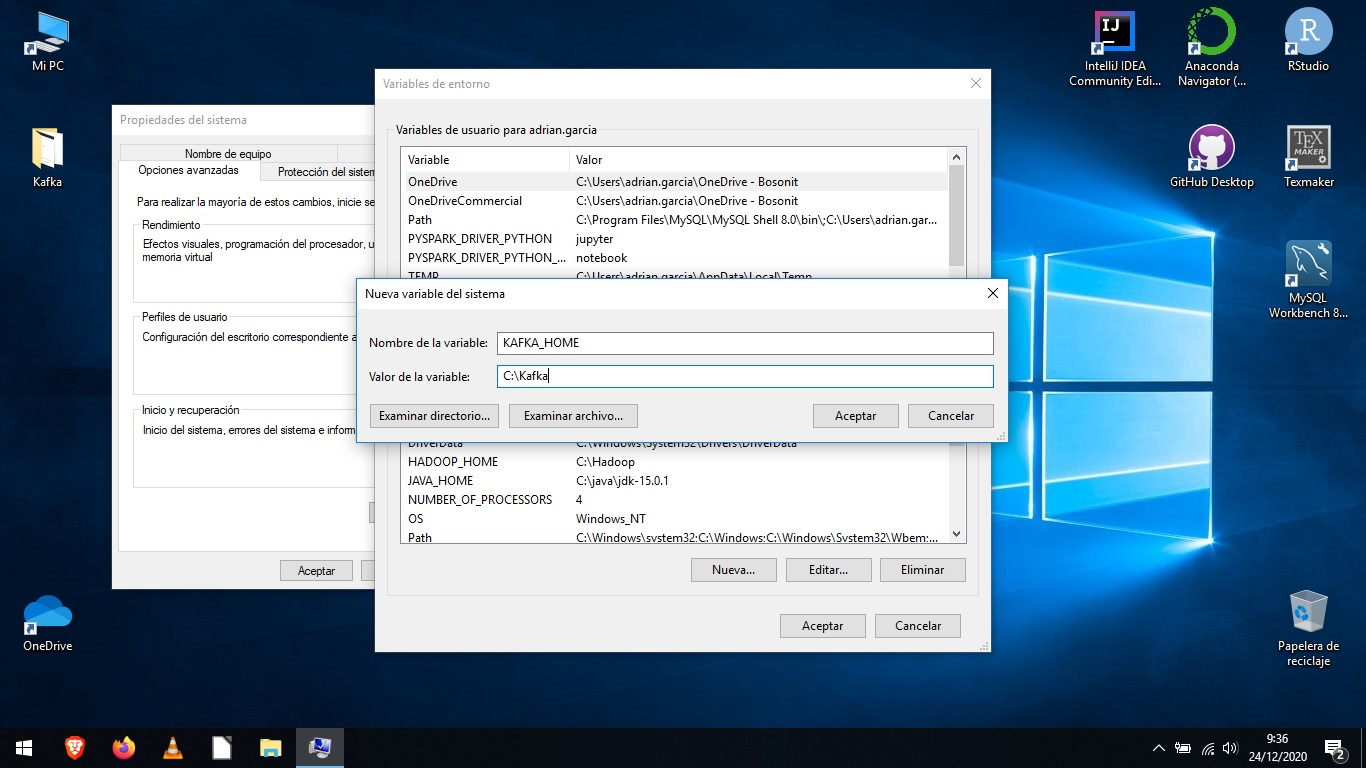
\includegraphics[width=450pt]{./fotos/Kafka/04.jpg}
\end{center}
\end{figure}

Hacemos clic en aceptar.

$\bullet$ PATH 

Si por alguna razón no tienes abierta la ventana de variables de entorno, repite los pasos anteriores. Ahora vamos a editar la variable Path que ya existe dentro de variables del sistema. La seleccionamos y le damos a editar:

\begin{figure}[H]
\begin{center}
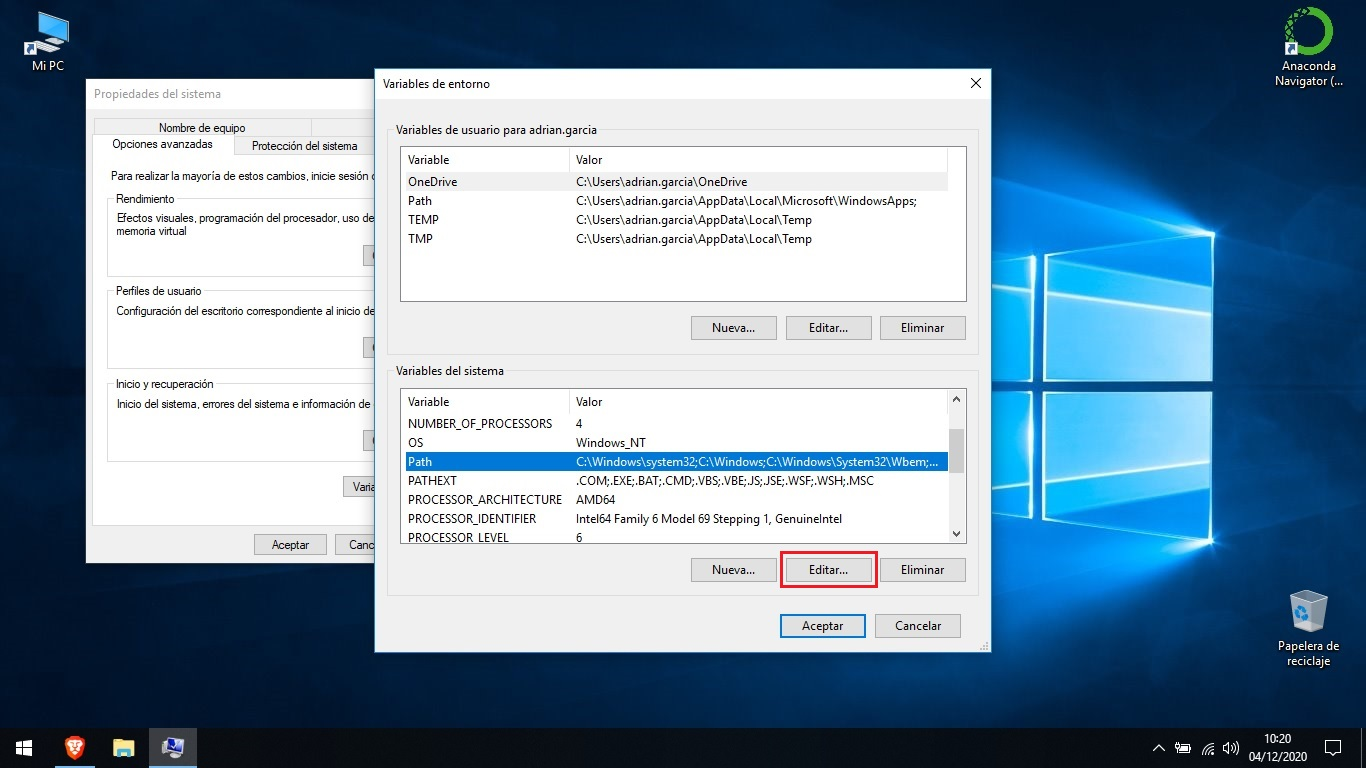
\includegraphics[width=450pt]{./fotos/introduccion/12 - Java (V).jpg}
\end{center}
\end{figure}

Podrás ver todos los valores que tiene por defecto la variable Path. No los modifiques o elimines, solo haz click en 'Nuevo' 

\begin{figure}[H]
\begin{center}
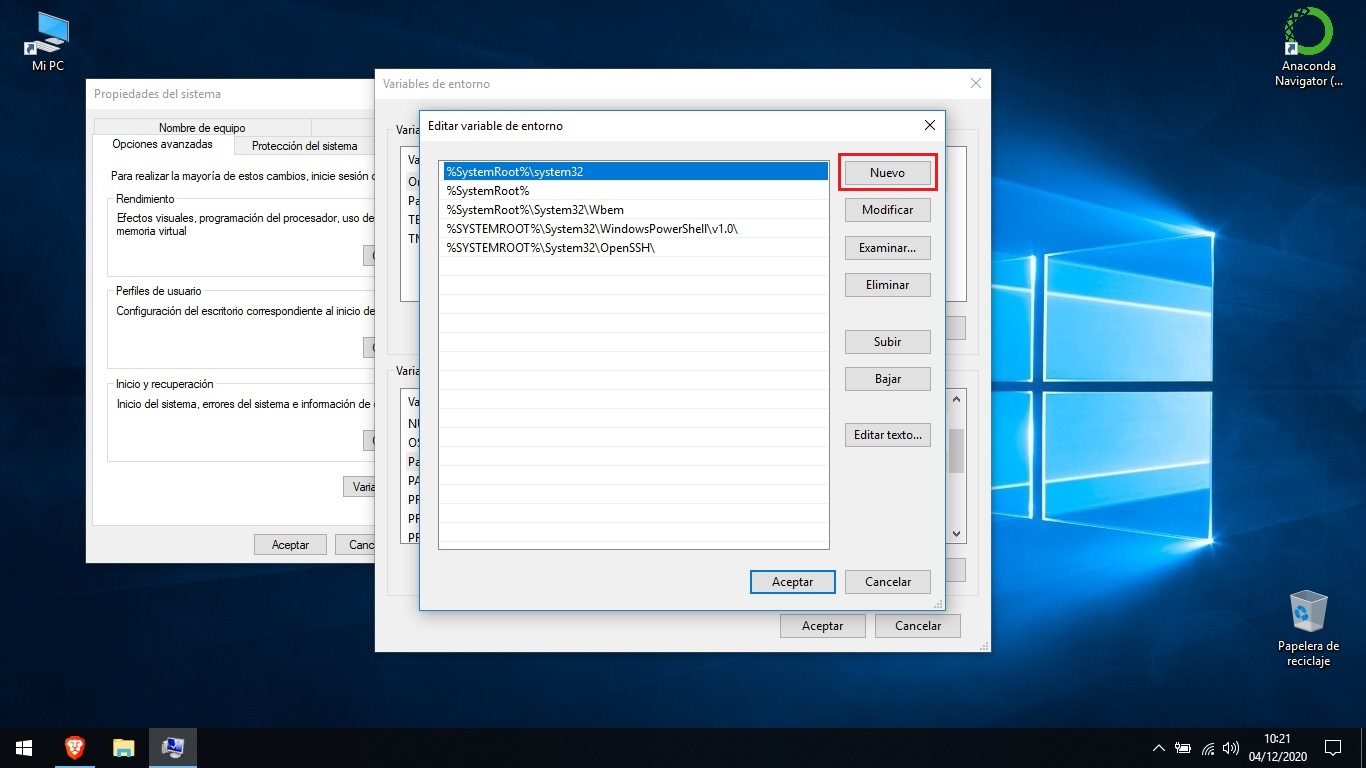
\includegraphics[width=450pt]{./fotos/introduccion/13 - Java (V).jpg}
\end{center}
\end{figure}

Escribiremos la ruta a la instalación de Kafka, pero en este caso direccionandolo a la carpeta windows dentro de la carpeta bin. Si has seguido todos los pasos de esta guia, la ruta sera \textit{C:/Kafka/bin/windows}

\begin{figure}[H]
\begin{center}
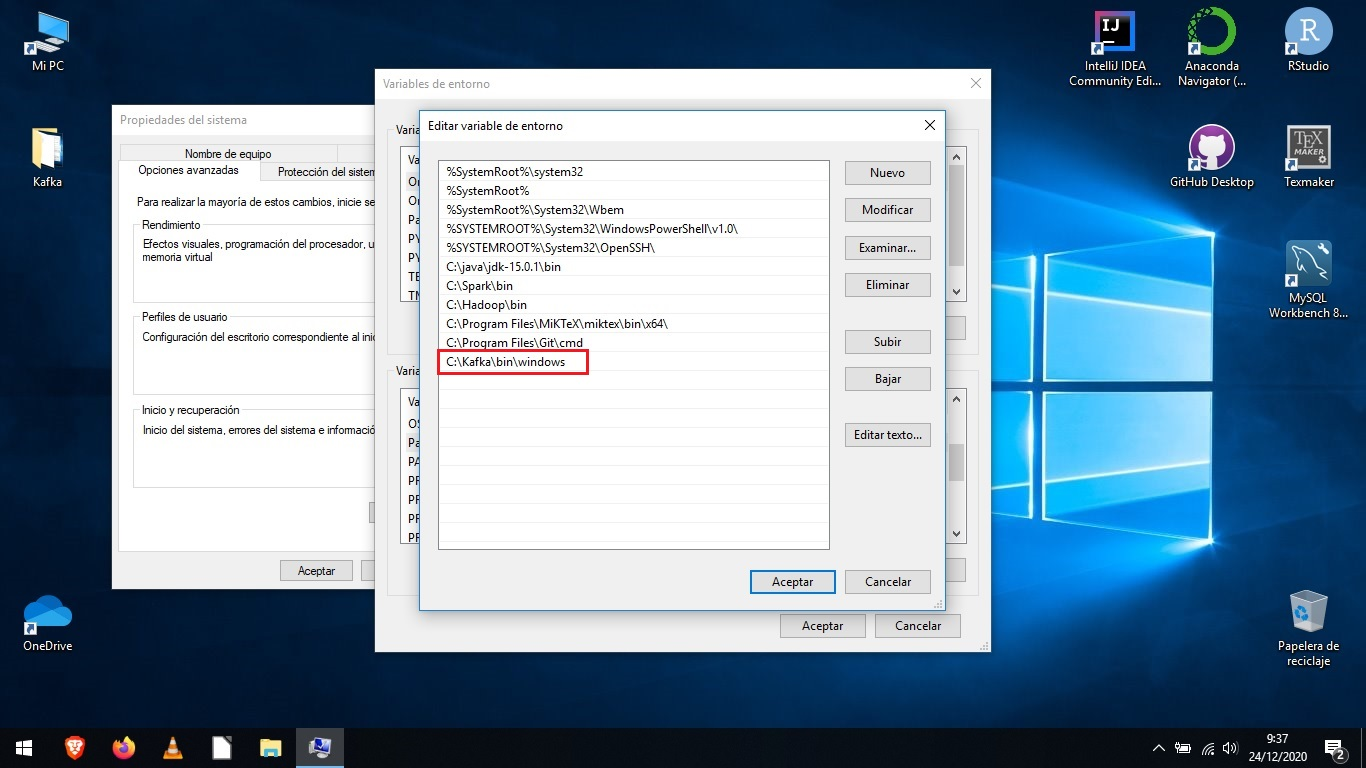
\includegraphics[width=450pt]{./fotos/Kafka/05 (V).jpg}
\end{center}
\end{figure}

Aceptamos en la ventana de Path y volvemos a aceptar en la ventana de variables de entorno y en propiedades del sistema.

\clearpage

\subsubsection{Verificación de Funcionamiento}

Ahora comprobaremos que la instalación se ha efectuado de forma correcta. Para ello abriremos una consola del sistema. Para ello le damos a inicio, escribiremos $\textit{cmd}$ y ejecutaremos \textit{Simbolo del sistema}. Lo primero que deberemos hacer sera inicializar Apache Zookeeper. Para ello escribiremos \textbf{C:\textbackslash Kafka\textbackslash bin\textbackslash windows\textbackslash zookeeper-server-start.bat C:\textbackslash Kafka\textbackslash config\textbackslash zookeeper.properties}:

\begin{figure}[H]
\begin{center}
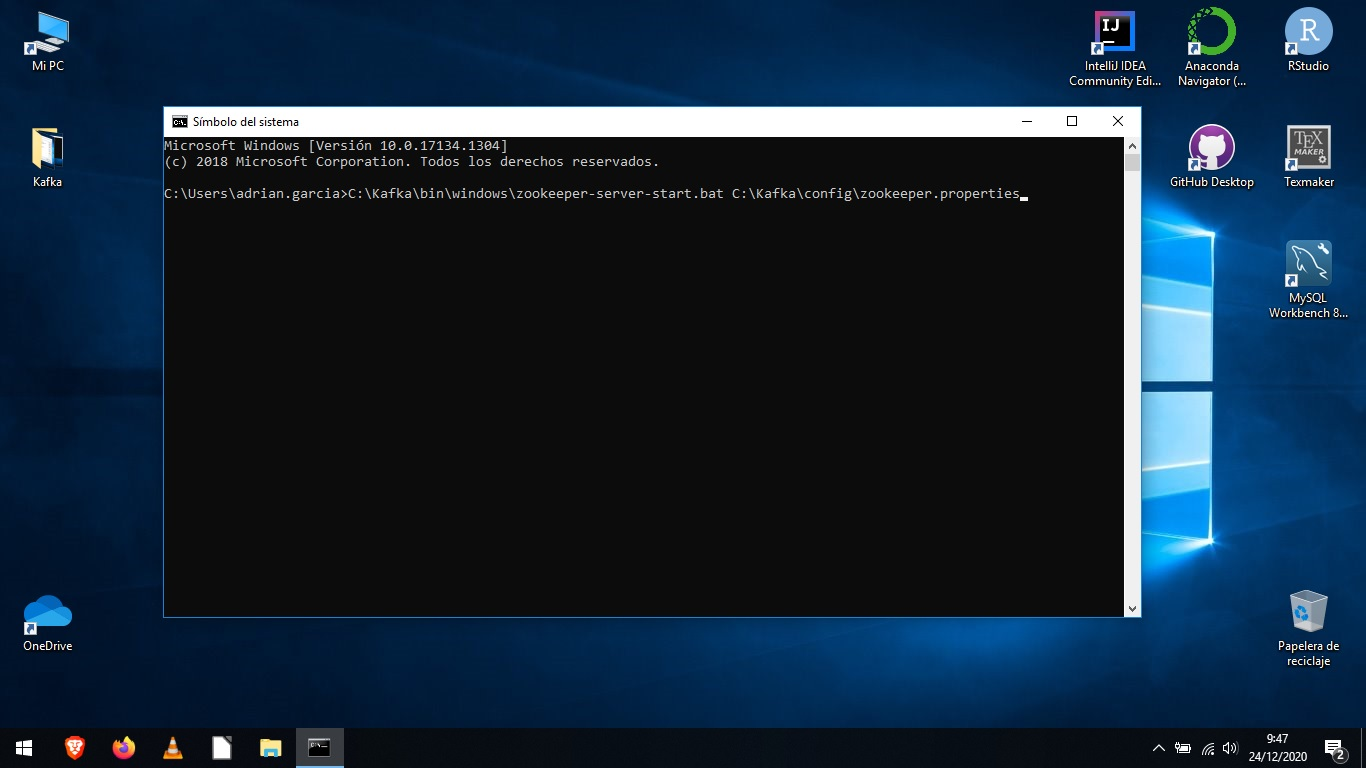
\includegraphics[width=450pt]{./fotos/Kafka/06.jpg}
\end{center}
\end{figure}

Al ejecutar este comando deberia salirnos algo similar a esto:

\begin{figure}[H]
\begin{center}
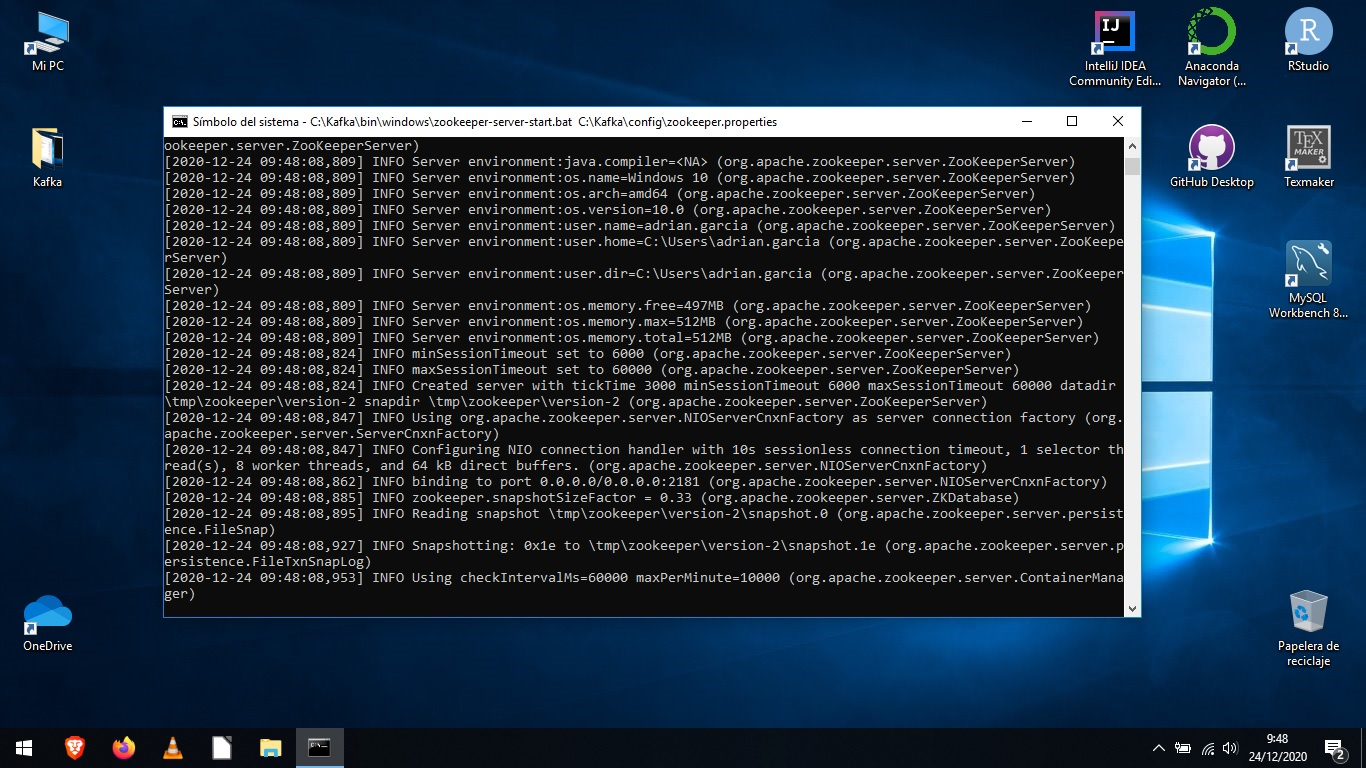
\includegraphics[width=450pt]{./fotos/Kafka/07.jpg}
\end{center}
\end{figure}

Ahora deberemos abrir otra consola del sistema \textbf{nueva} de la misma forma que antes y sin cerrar la consola donde hemos inicializado Apache Zookeeper. Ahora ejecutaremos Kafka Broker/Server. En este caso escribiremos \textbf{C:\textbackslash Kafka\textbackslash bin\textbackslash windows\textbackslash kafka-server-start.bat C:\textbackslash Kafka\textbackslash config\textbackslash server.properties}:

\begin{figure}[H]
\begin{center}
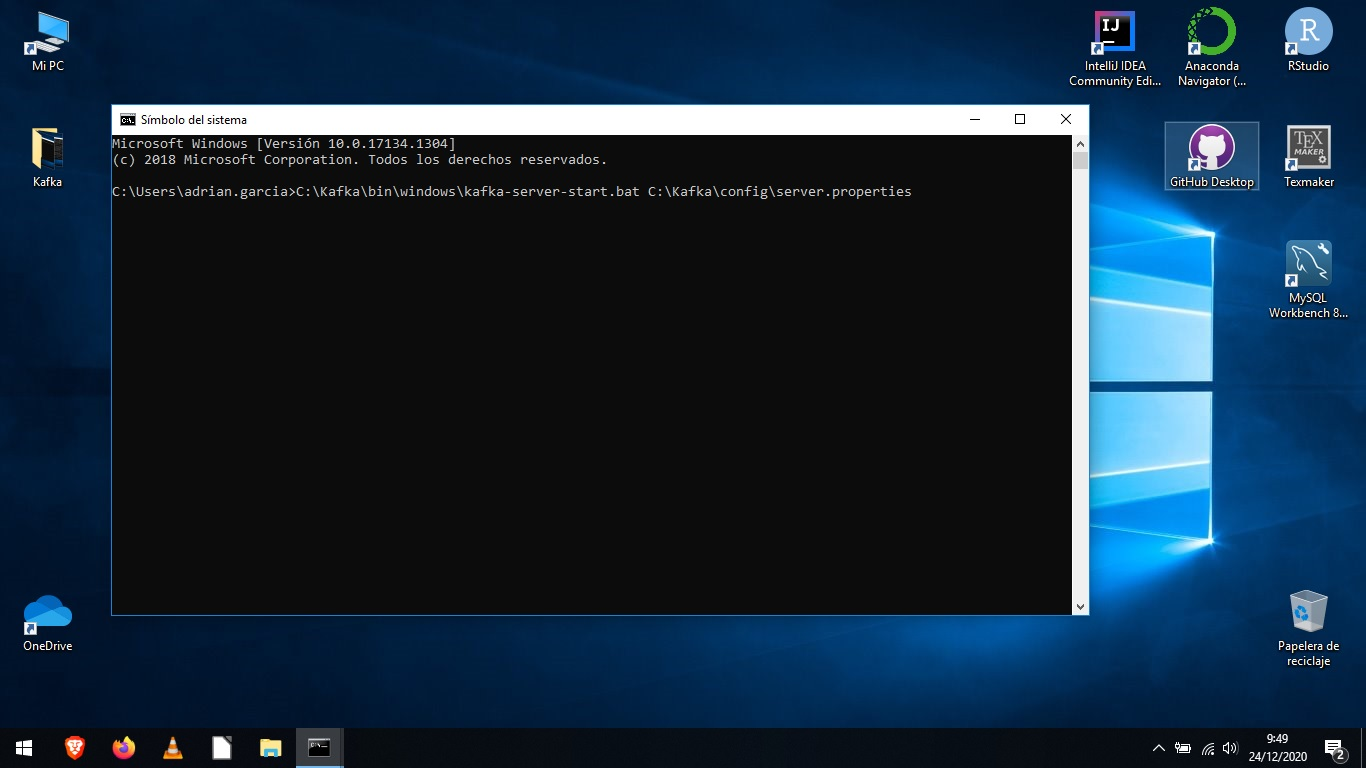
\includegraphics[width=450pt]{./fotos/Kafka/08.jpg}
\end{center}
\end{figure}

Y tambien deberiamos obtener algo similar a:

\begin{figure}[H]
\begin{center}
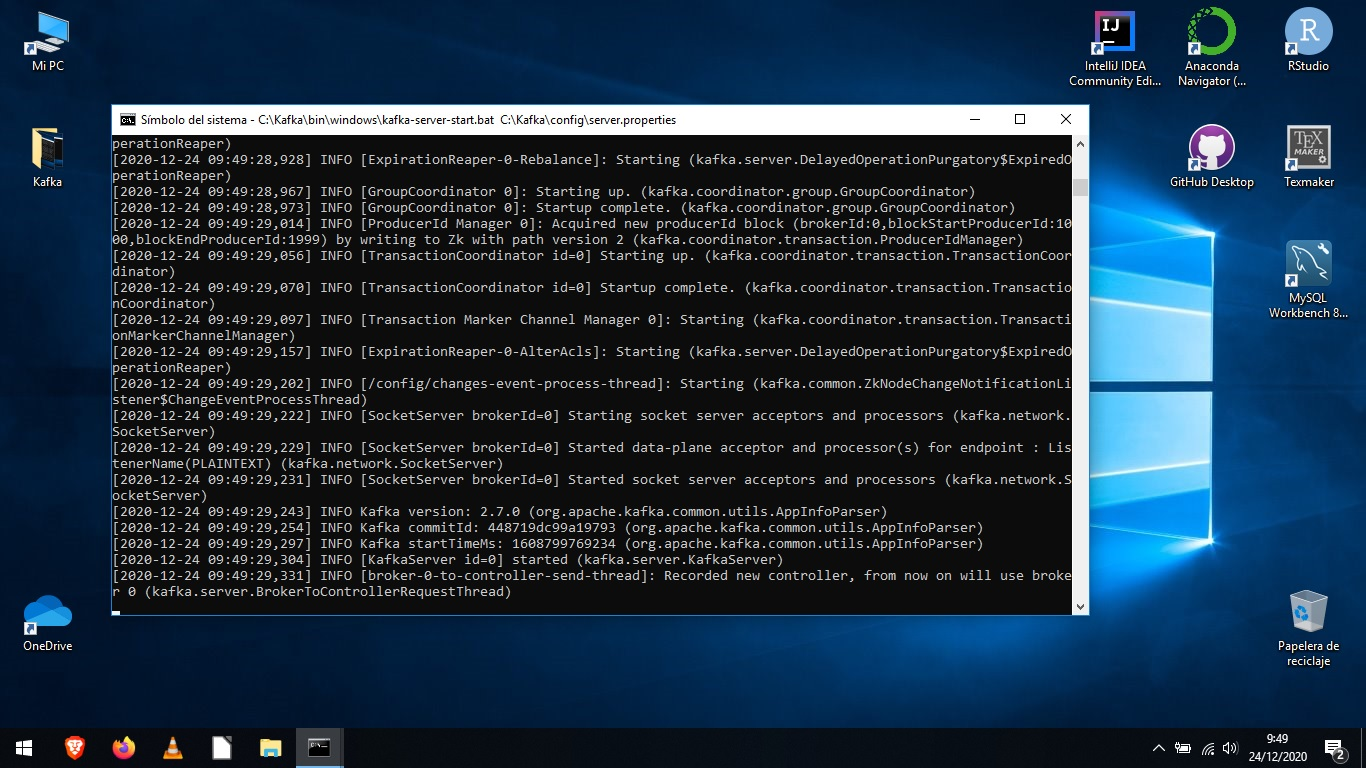
\includegraphics[width=450pt]{./fotos/Kafka/09.jpg}
\end{center}
\end{figure}

Ahora que tenemos Apache Zookeeper y Kafka Broker funcionando, sin cerrar ningun simbolo del sistema abriremos un tercero para probar que todo se ha ejecutado y funciona perfectamente.

\begin{figure}[H]
\begin{center}
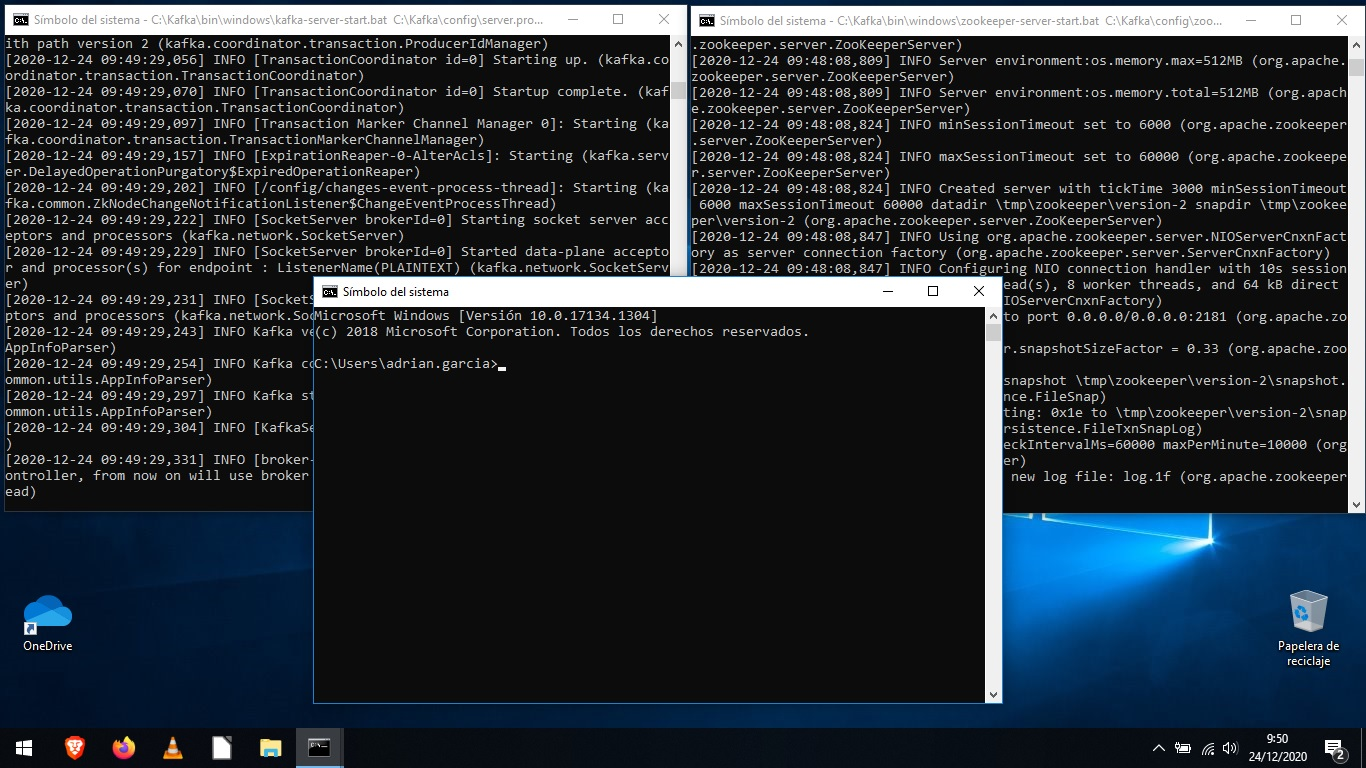
\includegraphics[width=450pt]{./fotos/Kafka/10.jpg}
\end{center}
\end{figure}

Primero solicitaremos que liste todos los topics, que en principio no deberiamos tener ninguno. Para ello escribiremos \textbf{C:\textbackslash Kafka\textbackslash bin\textbackslash windows\textbackslash kafka-topics.bat --list --zookeeper localhost:2181} 

\begin{figure}[H]
\begin{center}
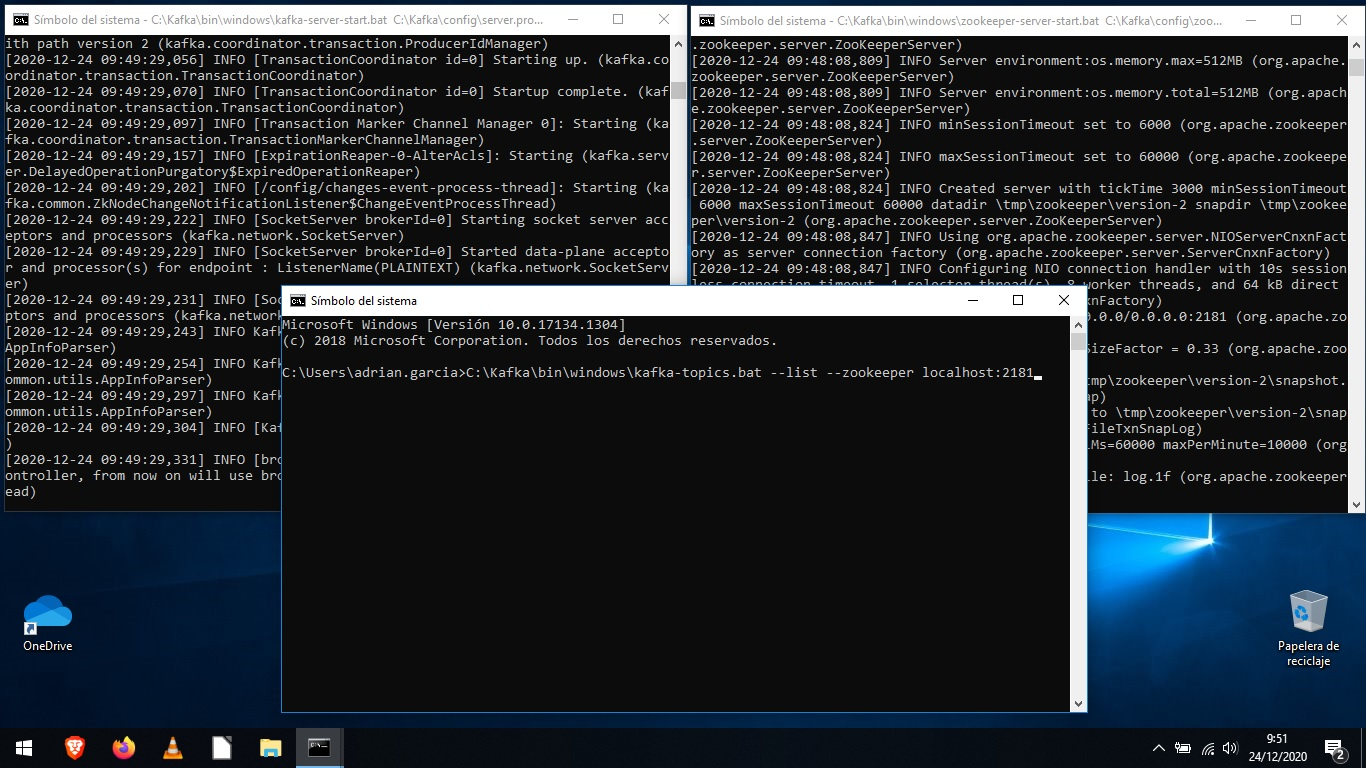
\includegraphics[width=450pt]{./fotos/Kafka/11.jpg}
\end{center}
\end{figure}

De la misma forma podemos ejecutar un comando de creacion de topics haciendo \textbf{C:\textbackslash Kafka\textbackslash bin\textbackslash windows\textbackslash kafka-topics.bat --create --zookeeper localhost:2181 --replication-factor 1 --partitions 100 --topic demo}. Y para mostrar las propiedades de este topic recien creado podemos hacer \textbf{C:\textbackslash Kafka\textbackslash bin\textbackslash windows\textbackslash kafka-topics.bat --describe --zookeeper localhost:2181 --topic demo}

\begin{figure}[H]
\begin{center}
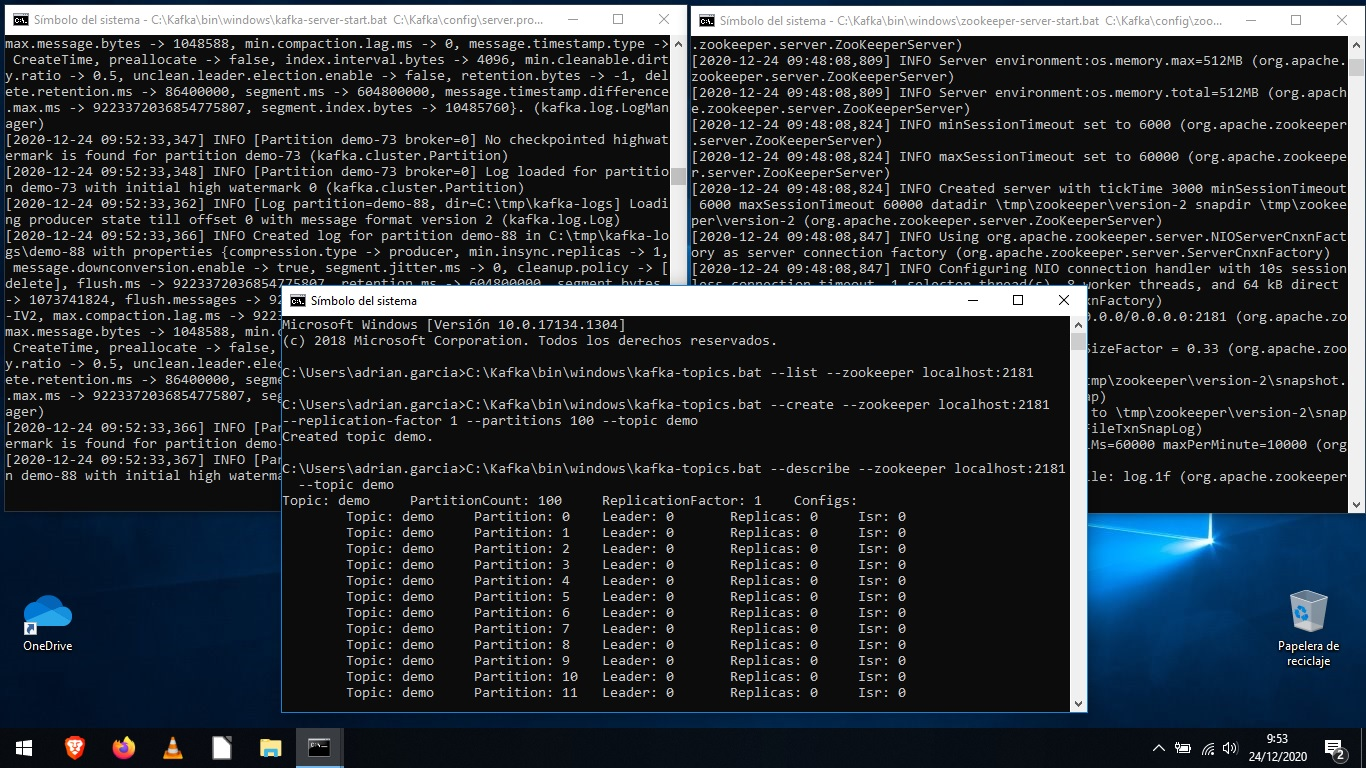
\includegraphics[width=450pt]{./fotos/Kafka/12.jpg}
\end{center}
\end{figure}

Para ver la lista de topics \textbf{C:\textbackslash Kafka\textbackslash bin\textbackslash windows\textbackslash kafka-topics.bat --list --zookeeper localhost:2181} y para eliminarlo \textbf{C:\textbackslash Kafka\textbackslash bin\textbackslash windows\textbackslash kafka-topics.bat --delete --zookeeper localhost:2181 --topic demo}

\begin{figure}[H]
\begin{center}
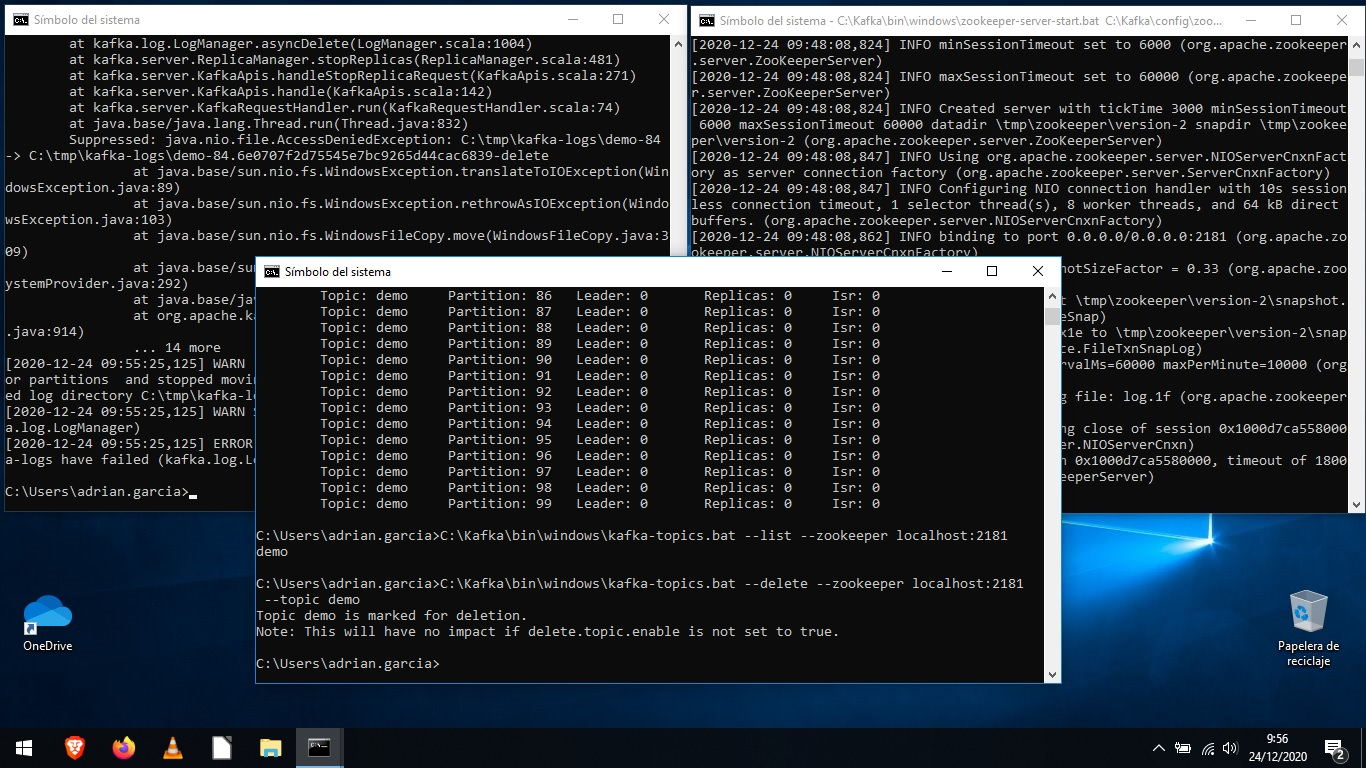
\includegraphics[width=450pt]{./fotos/Kafka/13.jpg}
\end{center}
\end{figure}

\section{Instalación y Configuración en Ubuntu}

\subsection{Requisitos}

Sistema operativo Ubuntu de 64bits

\clearpage

\subsection{Java JDK}

El Java JDK es el Java Development Kit, que traducido al español significa, Herramientas de desarrollo para Java. Aquí nos encontraremos con el compilador javac que es el encargado de convertir nuestro código fuente (.java) en bytecode (.class), el cual posteriormente sera interpretado y ejecutado en la JVM, Java Virtual Machine por sus siglas en ingles, que nuevamente en español significa, La Maquina Virtual de Java. 

Puede que nos suene mas Java JRE, este es el Java Runtime Environment, que en español significa, Entorno de Ejecución de Java. En palabras del propio portal de Java es la implementación de la Máquina virtual de Java que realmente ejecuta los programas de Java, esto quiere decir que aquí encontraremos todo lo necesario para ejecutar nuestras aplicaciones escritas en Java. 

Normalmente el JRE esta destinado a usuarios finales que no requieren el JDK, pues a diferencia de este, no contiene los programas necesarios para crear aplicaciones en el lenguaje Java, es así, que el JRE se puede instalar sin necesidad de instalar el JDK, pero al instalar el JDK, este siempre cuenta en su interior con el JRE.

\subsection{Anaconda}

Anaconda es una solución flexible de código abierto que proporciona las utilidades para crear, distribuir, instalar, actualizar y administrar software de manera multiplataforma. Ademas nos facilita la gestión de múltiples entornos de datos que se pueden mantener y ejecutar por separado sin interferencias entre sí.
 
Nos va a servir para el procesamiento de datos a gran escala, el análisis predictivo y la informática científica, que tiene como objetivo simplificar la gestión de empaquetado y distribución. Esta es quizás la Suite más completa para la Ciencia de datos con Python y que nos brinda una gran cantidad de funcionalidades que nos van a permitir desarrollar aplicaciones de una manera más eficiente, rápida y sencilla. 

\subsubsection{Instalación}

Para poder instalar la suite Anaconda necesitaremos el paquete CURL instalado en Ubuntu. Si es una instalacion limpia, abriremos una terminal y escribiremos:

\lstset{language=bash, breaklines=true, basicstyle=\ttfamily}
\begin{lstlisting}[frame=single]
sudo apt update
\end{lstlisting}

\clearpage

\section{Apache Spark}

\subsection{Tipos de administradores de clústers}

Actualmente (Version 3.0.2 de Spark), el sistema admite varios administradores de clusters:

$\bullet$ Standalone – un administrador de clúster simple incluido con Spark que facilita la configuracion de un cluster.

$\bullet$ Apache Mesos – un administrador de clúster general que también puede ejecutar Hadoop MapReduce y aplicaciones de servicio.

$\bullet$ Hadoop YARN – el administrador de recursos a partir de Hadoop 2.

$\bullet$ Kubernetes – un sistema de codigo abierto para automatizar el despliegue, el escalado y la gestion de aplicaciones en contenedores.

Existe un proyecto de terceros (no compatible con el proyecto Spark) para agregar compatibilidad con Nomad como administrador de clúster.





\section{Servicios en la nube}

\subsection{Databricks}

Databricks es el nombre de la plataforma analítica de datos basada en Apache Spark desarrollada por la compañía con el mismo nombre. La empresa se fundó en 2013 con los creadores y los desarrolladores principales de Spark. Permite hacer analítica Big Data e inteligencia artificial con Spark de una forma sencilla y colaborativa. Esta plataforma tambien está disponible como servicio cloud en Microsoft Azure y Amazon Web Services (AWS).

\subsubsection{Registro}

Databricks nos permite probar su funcionamiento con una serie de limitaciones por medio de la llamada 'Databricks Community Edition'. Lo primero que deberemos hacer para poder acceder a esta version de prueba sera entrar en la siguiente web:

\href{https://community.cloud.databricks.com/}{https://community.cloud.databricks.com/}

Al entrar veremos la siguiente pagina web:

\begin{figure}[H]
\begin{center}
\includegraphics[width=500pt]{./fotos/Databricks/1 - Databricks (V).jpg}
\end{center}
\end{figure}

Lo primero que deberemos hacer es registrarnos en la web para tener un nombre de usuario y contraseña. Para ello hacemos click en 'Sign Up' y completamos los datos que se nos solicitan en la web.

\begin{figure}[H]
\begin{center}
\includegraphics[width=500pt]{./fotos/Databricks/2 - Databricks (V).jpg}
\end{center}
\end{figure}

Una vez completado el registro y verificado nuestra direccion de email ya podemos iniciar sesion. Lo que encontraremos al iniciar sesion sera un Dashboard de esta manera:

\begin{figure}[H]
\begin{center}
\includegraphics[width=500pt]{./fotos/Databricks/3 - Databricks.jpg}
\end{center}
\end{figure}

\subsubsection{Creacion de Cluster}

Como podemos ver, se nos incluye una guia rapida y las principales funciones basicas. Lo que haremos ahora es ir a 'Clusters' en el menu lateral para crear nuestro Cluster personalizado.

\begin{figure}[H]
\begin{center}
\includegraphics[width=500pt]{./fotos/Databricks/4 - Databricks (V).jpg}
\end{center}
\end{figure}

\begin{figure}[H]
\begin{center}
\includegraphics[width=500pt]{./fotos/Databricks/5 - Databricks (V).jpg}
\end{center}
\end{figure}

Ahora haremos click en 'Create Cluster':

\begin{figure}[H]
\begin{center}
\includegraphics[width=500pt]{./fotos/Databricks/6 - Databricks (V).jpg}
\end{center}
\end{figure}

Como podemos ver en la imagen, en primer lugar se nos pide un nombre para nuestro cluster. Lo siguiente sera elegir que version del sistema queremos para nuestro cluster en el que se indicara la version de Scala y Spark que tendra. Si hacemos click en él, veremos un desplegable:

\begin{figure}[H]
\begin{center}
\includegraphics[width=500pt]{./fotos/Databricks/7 - Databricks (V).jpg}
\end{center}
\end{figure}

Veremos que ademas de las diferentes versiones del sistema, aparecen algunos subtitulos que tienen el siguiente significado:

$\bullet$ LTS: en ingles 'Long Term Support'. Es un termino informatico usado para nombrar versiones o ediciones de software diseñadas para tener soporte durante un periodo de tiempo mayor de lo normal. Se aplica normalmente a proyectos de software de codigo abierto. Es la mas recomendable si vamos a hacer un proyecto a largo plazo en el que no queramos quedarnos en algun momento sin soporte.

$\bullet$ ML: Como se dice en la documentacion de Databricks, las versiones con ML contiene las librerias de machine learning mas populares, incluyendo TensorFlow, Pytorch y XGBoost. Ademas tambien es compatible con deep learning distribuido usando Horovod. Se recomienda si vamos a usar tecnicas de machine learning.

$\bullet$ Beta: Version de prueba que esta en fase de pulido. Solo se recomienda si vamos a probar nuevas funcionalidades no incluidas en versiones anteriores mas estables.

En la parte derecha tambien veremos que existen versiones estandar y versiones que incluyen GPU. Estas versiones con GPU solo deben seleccionarse si vamos a utilizar el procesamiento en paralelo de estas.

Si necesitamos ampliar la informacion sobre las diferentes versiones que nos proporciona la plataforma podemos acceder a la web:

\href{https://docs.databricks.com/release-notes/runtime/releases.html}{https://docs.databricks.com/release-notes/runtime/releases.html}

En nuestro caso seleccionaremos la version 7.4 ML sin GPU, que incluye la version 2.12 de Scala y la 3.01 de Spark. 

\begin{figure}[H]
\begin{center}
\includegraphics[width=500pt]{./fotos/Databricks/8 - Databricks (V).jpg}
\end{center}
\end{figure}

La ultima opcion que vemos es la de 'Availability Zone' que nos indica donde estara hospedado nuestro cluster. Esto nos afectara en la velocidad entre envio de peticion y respuesta. En este caso solo tenemos opciones de Estados Unidos por lo que lo dejamos tal cual esta.

Una vez tenemos todas las caracteristicas deseadas solo tenemos que hacer click en 'Create Cluster'. El proceso de creacion puede tardar varios minutos, en cuanto este desplegado nuestro cluster veremos un indicador verde en la parte superior como en la siguiente imagen:

\begin{figure}[H]
\begin{center}
\includegraphics[width=500pt]{./fotos/Databricks/9 - Databricks (V).jpg}
\end{center}
\end{figure}

\subsubsection{Creacion y carga de Notebooks}

Ahora para poder trabajar con nuestro cluster tendremos que ir a la seccion 'workspace'  en el menu lateral. En el como podemos ver en las siguientes imagenes, podremos crear un nuevo notebook o importar uno.

\begin{figure}[H]
\begin{center}
\includegraphics[width=500pt]{./fotos/Databricks/11 - Databricks (V).jpg}
\end{center}
\end{figure}

\begin{figure}[H]
\begin{center}
\includegraphics[width=500pt]{./fotos/Databricks/10 - Databricks.jpg}
\end{center}
\end{figure}

Si le damos a importar se nos abrira una ventana donde podremos arrastrar el documento o seleccionarlo dentro de nuestro ordenador:

\begin{figure}[H]
\begin{center}
\includegraphics[width=500pt]{./fotos/Databricks/12 - Databricks.jpg}
\end{center}
\end{figure}

\begin{figure}[H]
\begin{center}
\includegraphics[width=500pt]{./fotos/Databricks/13 - Databricks.jpg}
\end{center}
\end{figure}

Entonces se nos abrira el notebook de la siguiente forma:

\begin{figure}[H]
\begin{center}
\includegraphics[width=500pt]{./fotos/Databricks/14 - Databricks.jpg}
\end{center}
\end{figure}

En la parte superior podremos seleccionar el cluster donde queremos que se ejecute el notebook, en nuestro caso solo tendremos una opcion:

\begin{figure}[H]
\begin{center}
\includegraphics[width=500pt]{./fotos/Databricks/15 - Databricks.jpg}
\end{center}
\end{figure}

Ahora que hemos seleccionado el cluster podemos comprobar que todo funciona como si estuvieramos programando en nuestro ordenador personal, solo que ahora el procesamiento se esta ejecutando remotamente en un cluster externo.

\begin{figure}[H]
\begin{center}
\includegraphics[width=500pt]{./fotos/Databricks/16 - Databricks (V).jpg}
\end{center}
\end{figure}

\clearpage

\subsection{Google Cloud}

De la misma forma que databricks nos ofrece el procesamiento en la nube. Google tambien dispone de su propia plataforma. Aunque tiene multitud de herramientas para distintos desarrollos y funciones diferentes, nos centraremos en como crear un almacenamiento permanente, inicializacion de cluster y creacion de notebooks.

\subsubsection{Registro}

Google Cloud nos ofrece con nuestra cuenta de gmail la opcion de probar todas las funciones de Google Cloud durante 1 año o hasta 300\$ de gasto. En este tipo de servicios, los gastos son en funcion de la utilizacion de recursos tanto de procesamiento como de almacenamiento. Para poder aprender a utilizar la plataforma y familiarizarnos con todas sus funciones la version de prueba nos sobra, ya que consumiremos antes el año que los 300\$.

Lo primero que tendremos que hacer sera registrarnos si no tenemos cuenta de Google o crear una. Una vez la tengamos iremos a la siguiente pagina web:

\begin{center}
\href{https://cloud.google.com/}{https://cloud.google.com/}
\end{center}

La pagina que nos aparecera sera la siguiente:

\begin{figure}[H]
\begin{center}
\includegraphics[width=500pt]{./fotos/GoogleCloud/1 - GC (V).jpg}
\end{center}
\end{figure}

Como podemos observar en la parte superior, ya se nos ofrece el servicio gratuito de prueba. Le damos a 'Empezar gratis' y nos pedira que iniciemos sesion.

\begin{figure}[H]
\begin{center}
\includegraphics[width=500pt]{./fotos/GoogleCloud/2 - GC.jpg}
\end{center}
\end{figure}

Ademas de aceptar las condiciones del servicio, se nos pedira un numero de tarjeta de credito. En ningun momento se nos cobrara nada, es simplemente como comprobacion de que es una persona fisica la que solicita el permiso y evitar duplicaciones de cuentas. Ademas al terminar el año no se cobrara nada, solo si se hace la actualizacion a version de pago de forma manual y explicita nos mantendran el servicio activo.

\begin{figure}[H]
\begin{center}
\includegraphics[width=500pt]{./fotos/GoogleCloud/4 - GC.jpg}
\end{center}
\end{figure}

Una vez hemos completado los pasos y hemos iniciado sesion la web principal sera asi:

\begin{figure}[H]
\begin{center}
\includegraphics[width=500pt]{./fotos/GoogleCloud/5 - GC.jpg}
\end{center}
\end{figure}

Donde ahora 'Empezar gratis' se ha convertido en 'Ir a la consola'. Hacemos click y nos llevara al Dashboard de la plataforma, donde tendremos que crear un proyecto haciendo click en 'Select project' en la parte superior:

\begin{figure}[H]
\begin{center}
\includegraphics[width=500pt]{./fotos/GoogleCloud/6 - GC (V).jpg}
\end{center}
\end{figure}

Solo tendremos que elegir un nombre para nuestro proyecto y abrirlo.

\begin{figure}[H]
\begin{center}
\includegraphics[width=500pt]{./fotos/GoogleCloud/7 - GC (V).jpg}
\end{center}
\end{figure}

Veremos que en la parte izquiera tendremos un menu con muchisimas opciones. Todo eso son diferentes funcionalidades y herramientas de las que dispone la plataforma de Google Cloud. 

\begin{figure}[H]
\begin{center}
\includegraphics[width=500pt]{./fotos/GoogleCloud/8 - GC (V).jpg}
\end{center}
\end{figure}

\subsubsection{Storage}

Cuando vamos a trabajar con clusters, tenemos que crear un lugar de almacenamiento permanente. Esto se debe a que cuando desplegamos el cluster, este se crea y se mantiene activo el tiempo que nosotros deseemos, pero una vez hemos terminado, el cluster y sus datos internos son eliminados. Para ello crearemos primero un almacenamiento permanente que funciona de forma similar a Google Drive, de esta forma cuando dejemos de trabajar y eliminemos nuestro cluster, los archivos permaneceran y podremos volver a crear otro cluster y continuar trabajando donde lo habiamos dejado.

Para ello iremos en el menu lateral a donde pone 'Storage' como podemos ver en la siguiente imagen:

\begin{figure}[H]
\begin{center}
\includegraphics[width=500pt]{./fotos/GoogleCloud/9 - GC (V).jpg}
\end{center}
\end{figure}

Recomiendo que hagais click en la chincheta (Pin) para que nos guarde la seccion Storage en la parte superior y no tener que buscarlo cada vez que queramos trabajar con el.

Una vez entramos veremos algo asi:

\begin{figure}[H]
\begin{center}
\includegraphics[width=500pt]{./fotos/GoogleCloud/10 - GC.jpg}
\end{center}
\end{figure}

Ahora crearemos nuestro Bucket donde almacenaremos los datos que queremos de forma permanente. Se nos ofreceran diferentes opciones como nombre, region donde queremos que se almacenen los datos, si queremos los datos centralizados o replicados en varias regiones, el tipo de acceso que haremos a el... 

En nuestro caso como podemos ver en las siguientes imagenes dejaremos todo por defecto, con las opciones mas simples. Solo modificaremos el apartado 'Location' donde seleccionaremos una region de Europa para minimizar el tiempo de acceso.

\begin{figure}[H]
\begin{center}
\includegraphics[width=500pt]{./fotos/GoogleCloud/11 - GC.jpg}
\end{center}
\end{figure}

\begin{figure}[H]
\begin{center}
\includegraphics[width=500pt]{./fotos/GoogleCloud/12 - GC.jpg}
\end{center}
\end{figure}

\begin{figure}[H]
\begin{center}
\includegraphics[width=500pt]{./fotos/GoogleCloud/13 - GC.jpg}
\end{center}
\end{figure}

\begin{figure}[H]
\begin{center}
\includegraphics[width=500pt]{./fotos/GoogleCloud/14 - GC.jpg}
\end{center}
\end{figure}

\begin{figure}[H]
\begin{center}
\includegraphics[width=500pt]{./fotos/GoogleCloud/15 - GC.jpg}
\end{center}
\end{figure}

Una vez creado veremos que ahora en la seccion principal aparece nuestro Bucket con el nombre que hemos seleccionado.

\begin{figure}[H]
\begin{center}
\includegraphics[width=500pt]{./fotos/GoogleCloud/16 - GC.jpg}
\end{center}
\end{figure}

Y si hacemos click en el nombre nos llevara a la seccion donde podremos configurarlo y subir archivos:

\begin{figure}[H]
\begin{center}
\includegraphics[width=500pt]{./fotos/GoogleCloud/16 - GC.jpg}
\end{center}
\end{figure}

\subsubsection{Dataproc}

Dataproc es un servicio en la nube rápido, fácil de usar y totalmente gestionado para ejecutar clústeres de Apache Spark y Apache Hadoop de una manera rapida y sencilla.

De la misma forma que en la seccion anterior, buscaremos en el menu izquierdo la seccion 'Dataproc', igual que antes, tambien recomiendo fijarla por medio de la chincheta. 

La primera vez que hagamos click seguramente se nos solicite activar la API, aceptamos y nos llevara a la siguiente pantalla:

\begin{figure}[H]
\begin{center}
\includegraphics[width=500pt]{./fotos/GoogleCloud/21 - GC.jpg}
\end{center}
\end{figure}

Hacemos click en 'Enable', esperamos y ya podemos continuar en la siguiente pantalla:

\begin{figure}[H]
\begin{center}
\includegraphics[width=500pt]{./fotos/GoogleCloud/22 - GC.jpg}
\end{center}
\end{figure}

Aqui veremos de forma similar a la web de Databricks que sera donde crearemos y gestionaremos el cluster. Le damos a 'Create Cluster' y nos llevara a la pagina de configuracion:

\begin{figure}[H]
\begin{center}
\includegraphics[width=500pt]{./fotos/GoogleCloud/23 - GC.jpg}
\end{center}
\end{figure}

De forma similar al resto de plataformas, se nos solicitara el nombre del cluster, la region en la que queremos que sea desplegado y el tipo de cluster. 

Como ya sabemos, existen diferentes tipos de cluster. En nuestro caso seleccionaremos la version de un 1 Master y N Workers. 

Tambien se nos da la opcion de activar que autoescale, es decir, que aumente el numero de Workers segun aumente la solicitud de procesamiento. En nuestro caso no va a ser necesario.

Si seguimos bajando veremos el tipo de sistema operativo que queremos que tenga el cluster y podremos desplegar todos los disponibles:

\begin{figure}[H]
\begin{center}
\includegraphics[width=500pt]{./fotos/GoogleCloud/24 - GC.jpg}
\end{center}
\end{figure}

\begin{figure}[H]
\begin{center}
\includegraphics[width=500pt]{./fotos/GoogleCloud/25 - GC.jpg}
\end{center}
\end{figure}

En nuestro caso recomendamos seleccionar la version 1.4 que incluye el sistema operativo Debian 10 con Hadoop 2.9 y Spark 2.4.

En la ultima seccion veremos los componentes que queremos incluir en nuestro cluster, que en nuestro caso hemos seleccionado Anaconda y Jupiter Notebook. Y no nos olvidemos de marcar 'Enable component gateway' para poder trabajar sin errores en el navegador.

\begin{figure}[H]
\begin{center}
\includegraphics[width=500pt]{./fotos/GoogleCloud/26 - GC.jpg}
\end{center}
\end{figure}

En el segundo apartado de la configuracion veremos y podremos modificar las caracteristicas del Master y los Workers:

\begin{figure}[H]
\begin{center}
\includegraphics[width=500pt]{./fotos/GoogleCloud/27 - GC.jpg}
\end{center}
\end{figure}

Para el Master vamos a seleccionar el mas pequeño ya que para nuestro aprendizaje no vamos a necesitar una gran cantidad de potencia de calculo y las caracteristicas por defecto en cuanto a tamaño de disco y tipo de disco:

\begin{figure}[H]
\begin{center}
\includegraphics[width=500pt]{./fotos/GoogleCloud/28 - GC.jpg}
\end{center}
\end{figure}

Si bajamos vemos la seccion de Workers, donde podremos seleccionar cuantos queremos, la capacidad de cada uno de ellos y el tamaño de disco y tipo de disco. En mi caso como en el Master selecciono el de menos potencia y pongo el tamaño de los discos a 100. De todas formas se puede dejar por defecto sin ningun problema.

\begin{figure}[H]
\begin{center}
\includegraphics[width=500pt]{./fotos/GoogleCloud/29 - GC.jpg}
\end{center}
\end{figure}

En la tercera seccion vamos a dejar la primera parte de la siguiente manera por defecto:

\begin{figure}[H]
\begin{center}
\includegraphics[width=500pt]{./fotos/GoogleCloud/30 - GC.jpg}
\end{center}
\end{figure}

Y en la parte de abajo debemos fijarnos en activar la funcion de apagado tras un periodo de inactividad (2h en mi caso) para que el cluster se elimine cuando dejemos de usaro, por si se nos olvida apagarlo.

\begin{figure}[H]
\begin{center}
\includegraphics[width=500pt]{./fotos/GoogleCloud/31 - GC.jpg}
\end{center}
\end{figure} 

Pero aun mas importante es seleccionar 'Cloud Storage staging Bucket'. Aqui es donde seleccionaremos el Bucket que hemos creado en la seccion anterior y donde guardaremos nuestros Dataset y Notebooks para que el cluster pueda trabajar con ellos y queden guardados aunque el cluster sea eliminado. Lo seleccionamos asi:

\begin{figure}[H]
\begin{center}
\includegraphics[width=500pt]{./fotos/GoogleCloud/32 - GC.jpg}
\end{center}
\end{figure}

Y deeberia quedarnos algo asi:

\begin{figure}[H]
\begin{center}
\includegraphics[width=500pt]{./fotos/GoogleCloud/33 - GC.jpg}
\end{center}
\end{figure}

En la ultima seccion no tenemos que tocar nada:

\begin{figure}[H]
\begin{center}
\includegraphics[width=500pt]{./fotos/GoogleCloud/34 - GC.jpg}
\end{center}
\end{figure}

Solo darle a 'CREATE' y esperar a que se despliegue ya que suele tardar unos pocos minutos. Una vez ha sido creado nos saldra algo asi:

\begin{figure}[H]
\begin{center}
\includegraphics[width=500pt]{./fotos/GoogleCloud/35 - GC.jpg}
\end{center}
\end{figure}

Si hacemos click en el nombre del Cluster nos llevara a la informacion general donde podremos ver la monitorizacion de los procesos y usos del cluster.

\begin{figure}[H]
\begin{center}
\includegraphics[width=500pt]{./fotos/GoogleCloud/36 - GC.jpg}
\end{center}
\end{figure}

Pero lo importante es la seccion 'WEB INTERFACES' donde accederemos a los componentes instalados como Jupiter Notebook.
 
\begin{figure}[H]
\begin{center}
\includegraphics[width=500pt]{./fotos/GoogleCloud/37 - GC.jpg}
\end{center}
\end{figure}

Hacemos click en 'JupiterLab' y veremos lo siguiente:

\begin{figure}[H]
\begin{center}
\includegraphics[width=500pt]{./fotos/GoogleCloud/38 - GC.jpg}
\end{center}
\end{figure}

En la parte izquierda veremos dos carpetas, una GCS que es 'Google Cloud Storage' que se trata del almacenamiento permanente del que hablamos y Local que es el almacenamiento del propio cluster donde si entramos podremos ver los diferentes archivos del sistema operativo y demas del propio cluster. Esta carpeta Local es la que se eliminara al borrar el Cluster, por eso nos interesa almacenar todo en GCS.

Si entramos en la carpeta GCS podremos subir un notebook de prueba:

\begin{figure}[H]
\begin{center}
\includegraphics[width=500pt]{./fotos/GoogleCloud/39 - GC.jpg}
\end{center}
\end{figure}

Y quedara de la siquiente manera:

\begin{figure}[H]
\begin{center}
\includegraphics[width=500pt]{./fotos/GoogleCloud/40 - GC.jpg}
\end{center}
\end{figure}

Este archivo quedara guardado de forma permanente en Storage hasta que lo eliminemos manualmente, independientemente de que el cluster este activo o no.

Ahora vamos a subir un Dataset para poder comprobar que todo funciona correctamente. Si intentamos subirlo desde aqui nos dira que solo podemos subir archivos con un tamaño maximo de 15Mb por lo tanto vamos a volver a la seccion 'Storage':

\begin{figure}[H]
\begin{center}
\includegraphics[width=500pt]{./fotos/GoogleCloud/42 - GC.jpg}
\end{center}
\end{figure}

Entramos en la carpeta 'bosonit' que habiamos creado y veremos:

\begin{figure}[H]
\begin{center}
\includegraphics[width=500pt]{./fotos/GoogleCloud/41 - GC.jpg}
\end{center}
\end{figure}

Crearemos una carpeta dandole a 'Create Folder' y le pondremos de nombre data:

\begin{figure}[H]
\begin{center}
\includegraphics[width=500pt]{./fotos/GoogleCloud/43 - GC.jpg}
\end{center}
\end{figure}

\begin{figure}[H]
\begin{center}
\includegraphics[width=500pt]{./fotos/GoogleCloud/44 - GC.jpg}
\end{center}
\end{figure}

Entramos en ella y haciendo click en Upload subiremos nuestro dataset:

\begin{figure}[H]
\begin{center}
\includegraphics[width=500pt]{./fotos/GoogleCloud/45 - GC.jpg}
\end{center}
\end{figure}

\begin{figure}[H]
\begin{center}
\includegraphics[width=500pt]{./fotos/GoogleCloud/46 - GC.jpg}
\end{center}
\end{figure}

Ahora si volvemos a nuestro Notebook anterior y entramos en el:

\begin{figure}[H]
\begin{center}
\includegraphics[width=500pt]{./fotos/GoogleCloud/47 - GC.jpg}
\end{center}
\end{figure}

Arriba a la derecha seleccionaremos el kernel que queremos utilizar, en nuestro caso Pyspark:

\begin{figure}[H]
\begin{center}
\includegraphics[width=500pt]{./fotos/GoogleCloud/48 - GC.jpg}
\end{center}
\end{figure}

Y probaremos que todo funciona de la siguiente manera:

\begin{figure}[H]
\begin{center}
\includegraphics[width=500pt]{./fotos/GoogleCloud/49 - GC.jpg}
\end{center}
\end{figure}

Como puedes apreciar, la ruta para acceder a los datos almacenados en Storage tienen la ruta: gs://bosonit/data/dataset.csv , donde como vemos la ruta raiz es gs:// y luego el nombre del bucket, seguido de la carpeta data creada anteriormente y el nombre del dataset.

\section{Optimización}

\subsection{Elegir un tipo de compresión}

La elección de un cierto tipo de compresion y formato puede tener un impacto importante en el rendimiento. Hay tres importantes lugares donde considerar la compresion de los datos, son los trabajos de MapReduce y Spark Jobs, los datos almacenados en HBase y las queries de Impala. En la mayoria de los casos, los principios son similares para cada uno.

Cuando debamos decidir el formato y compresion a utilizar, debemos equilibrar la capacidad de procesamiento (CPU) necesario en la compresion y descompresion, la E/S del disco al leer o escribir datos y el ancho de banda necesario para enviar los datos a traves de la red. El equilibrio de estos factores depende de las caracteristicas especificas del clúster y de los datos, asi como del patron de uso de estos.

Por supuesto, la compresion no es recomendable cuando los datos ya tienen una cierta compresion (por ejemplo imagenes en formato JPEG). Es mas, el archivo comprimido puede ser mayor que el original.

Los formatos mas comunes de compresión son los siguientes:

\begin{figure}[H]
\centering
\includegraphics[width=500pt]{./fotos/eleccioncompresion.jpg}
\caption{Tabla 5.1 de Hadoop The Definitive Guide 4th Edition}
\end{figure}

\begin{itemize}

\item \textbf{GZIP} este formato de compresion usa mas recursos de la CPU que Snappy o LZO, pero proporciona una relación de compresión más alta. GZip es una buena opcion para datos en frio, a los que se accede con poca frecuencia. Snappy o LZO son una mejor opcion para datos en caliente, a los que se accede de forma frecuente. Como detalle, el formato GZIP comprime los datos hasta un 30\% mas que Snappy y usa 2 veces mas CPU cuando se leen en comparación con la lectura de un archivo en formato Snappy. 

\item \textbf{BZip2} puede conseguir más compresión que GZip para algunos tipos de datos, a costa de una menor velocidad de compresión y descompresión. HBase no soporta Bzip2.

\item \textbf{LZO} se enfoca en una mayor velocidad de descompresion y bajo uso de CPU y una mayor compresión a costa de mas consumo CPU. Los archivos LZO no se pueden dividir de forma nativa, pero existe el proyecto \href{https://www.anaconda.com/}{Hadoop-LZO} que hace posible la divisibilidad de este formato.

\item \textbf{Snappy} a menudo funciona mejor que LZO. Merece la pena realizar pruebas para ver si se detecta una diferencia significativa.

\item \textbf{Divisibilidad} \textit{Para MapReduce y Spark, es necesario que los datos comprimidos se puedan dividir, y los formatos BZip2 y LZO no son divisibles. Los bloques Snappy y GZip tampoco son divisibles, pero los archivos con bloques Snappy dentro de un formato de archivo contenedor como SequenceFile, Avro o Parquet si se pueden dividir. Snappy ademas esta diseñado para usarse con un formato contenedor, como SequenceFiles, archivos de datos Avro o Parquet, en lugar de usarse directamente en texto plano sin formato, por ejemplo, este ultimo no se puede dividir y por lo tanto no se puede procesar en paralelo. En el caso de datos para HBase, la capacidad de division no es relevante.}

\clearpage

Para MapReduce se pueden comprimir los datos intermedios, los de salida o ambos. Debemos ajustar los parametros que añadimos al job de MapReduce en consecuencia. Los siguientes ejemplos comprimen tanto los datos intermedios como los de salida. MR2 se muestra primero, seguido de MR1.
  
\begin{itemize}
	\item MRv2
	
	\lstset{language=Bash, breaklines=true, basicstyle=\footnotesize}
	\begin{lstlisting}[frame=single]
	hadoop jar hadoop-examples-.jar sort "-Dmapreduce.compress.map.output=true"
	"-Dmapreduce.map.output.compression.codec=org.apache.hadoop.io.compress.GzipCodec"
	"-Dmapreduce.output.compress=true"
	"-Dmapreduce.output.compression.codec=org.apache.hadoop.io.compress.GzipCodec" -outKey
	org.apache.hadoop.io.Text -outValue org.apache.hadoop.io.Text input output
	\end{lstlisting}
	
	\item MRv1

	\lstset{language=Bash, breaklines=true, basicstyle=\footnotesize}
	\begin{lstlisting}[frame=single]
	hadoop jar hadoop-examples-.jar sort "-Dmapred.compress.map.output=true"
	"-Dmapred.map.output.compression.codec=org.apache.hadoop.io.compress.GzipCodec"
	"-Dmapred.output.compress=true"
	"-Dmapred.output.compression.codec=org.apache.hadoop.io.compress.GzipCodec" -outKey
	org.apache.hadoop.io.Text -outValue org.apache.hadoop.io.Text input output
	\end{lstlisting}
	
\end{itemize}
\end{itemize}






\end{document}
